
På baggrund af simuleringer med Inundation Modellen og analysering af resultaterne præsenteres resultaterne for projektet i dette afsnit med ...

\subsection{Resultatet af simuleringen af oktober 2023 stormfloden}
I dette afsnit bliver der præsenteret resultaterne fra Inundation Modellen samt oversvømmelseskort fra studiekommunerne og hvilke arealanvendelser der blev påvirket.\\

I figur \ref{Subfig: Model Aabenraa} ses resultatet af Inundation Modellen for simuleringen af oktober 2023 stormfloden for Aabenraa og figur \ref{Subfig: Målt Aabenraa} viser det oversvømmelseskort Aabenraa kommune har udarbejdet der viser den reelle oversvømmelse. \\
Der er tydelige forskelle mellem de to resultater. Modellens resultat er større især vest for lystbådhavnen ved et større rekreativt område. Modellen resulterede i et areal på 1297614 m\textsuperscript{2}, mens det målte areal var på 707128 m\textsuperscript{2}. Dette resulterer i at modellens resultat er 83,5\% større end den målte hændelse. \\
Denne forskel skyldes primært de beredskabstiltag der blev indført om eftermiddagen den 20. oktober 2023 langs den sydlige strækning af industrihavnen. Disse beredsskabstiltag inkluderede en 1 km lang watertube og sandsække. Watertuben bristede under pres, men vandet blev standset af sandsække. 
Der er derimod også to områder hvor den målte oversvømmelse fandt sted, men hvor modellen ikke indikerede en oversvømmelse. Dette er to små vandløb syd for Aabenraa by. I den målte oversvømmelse er vandet trængt ind i små vandløb, mens i modellens resultat er de ikke blevet oversvømmet.    
\begin{figure}[H]
    \begin{subfigure}[t]{0.5\textwidth}
        \centering
        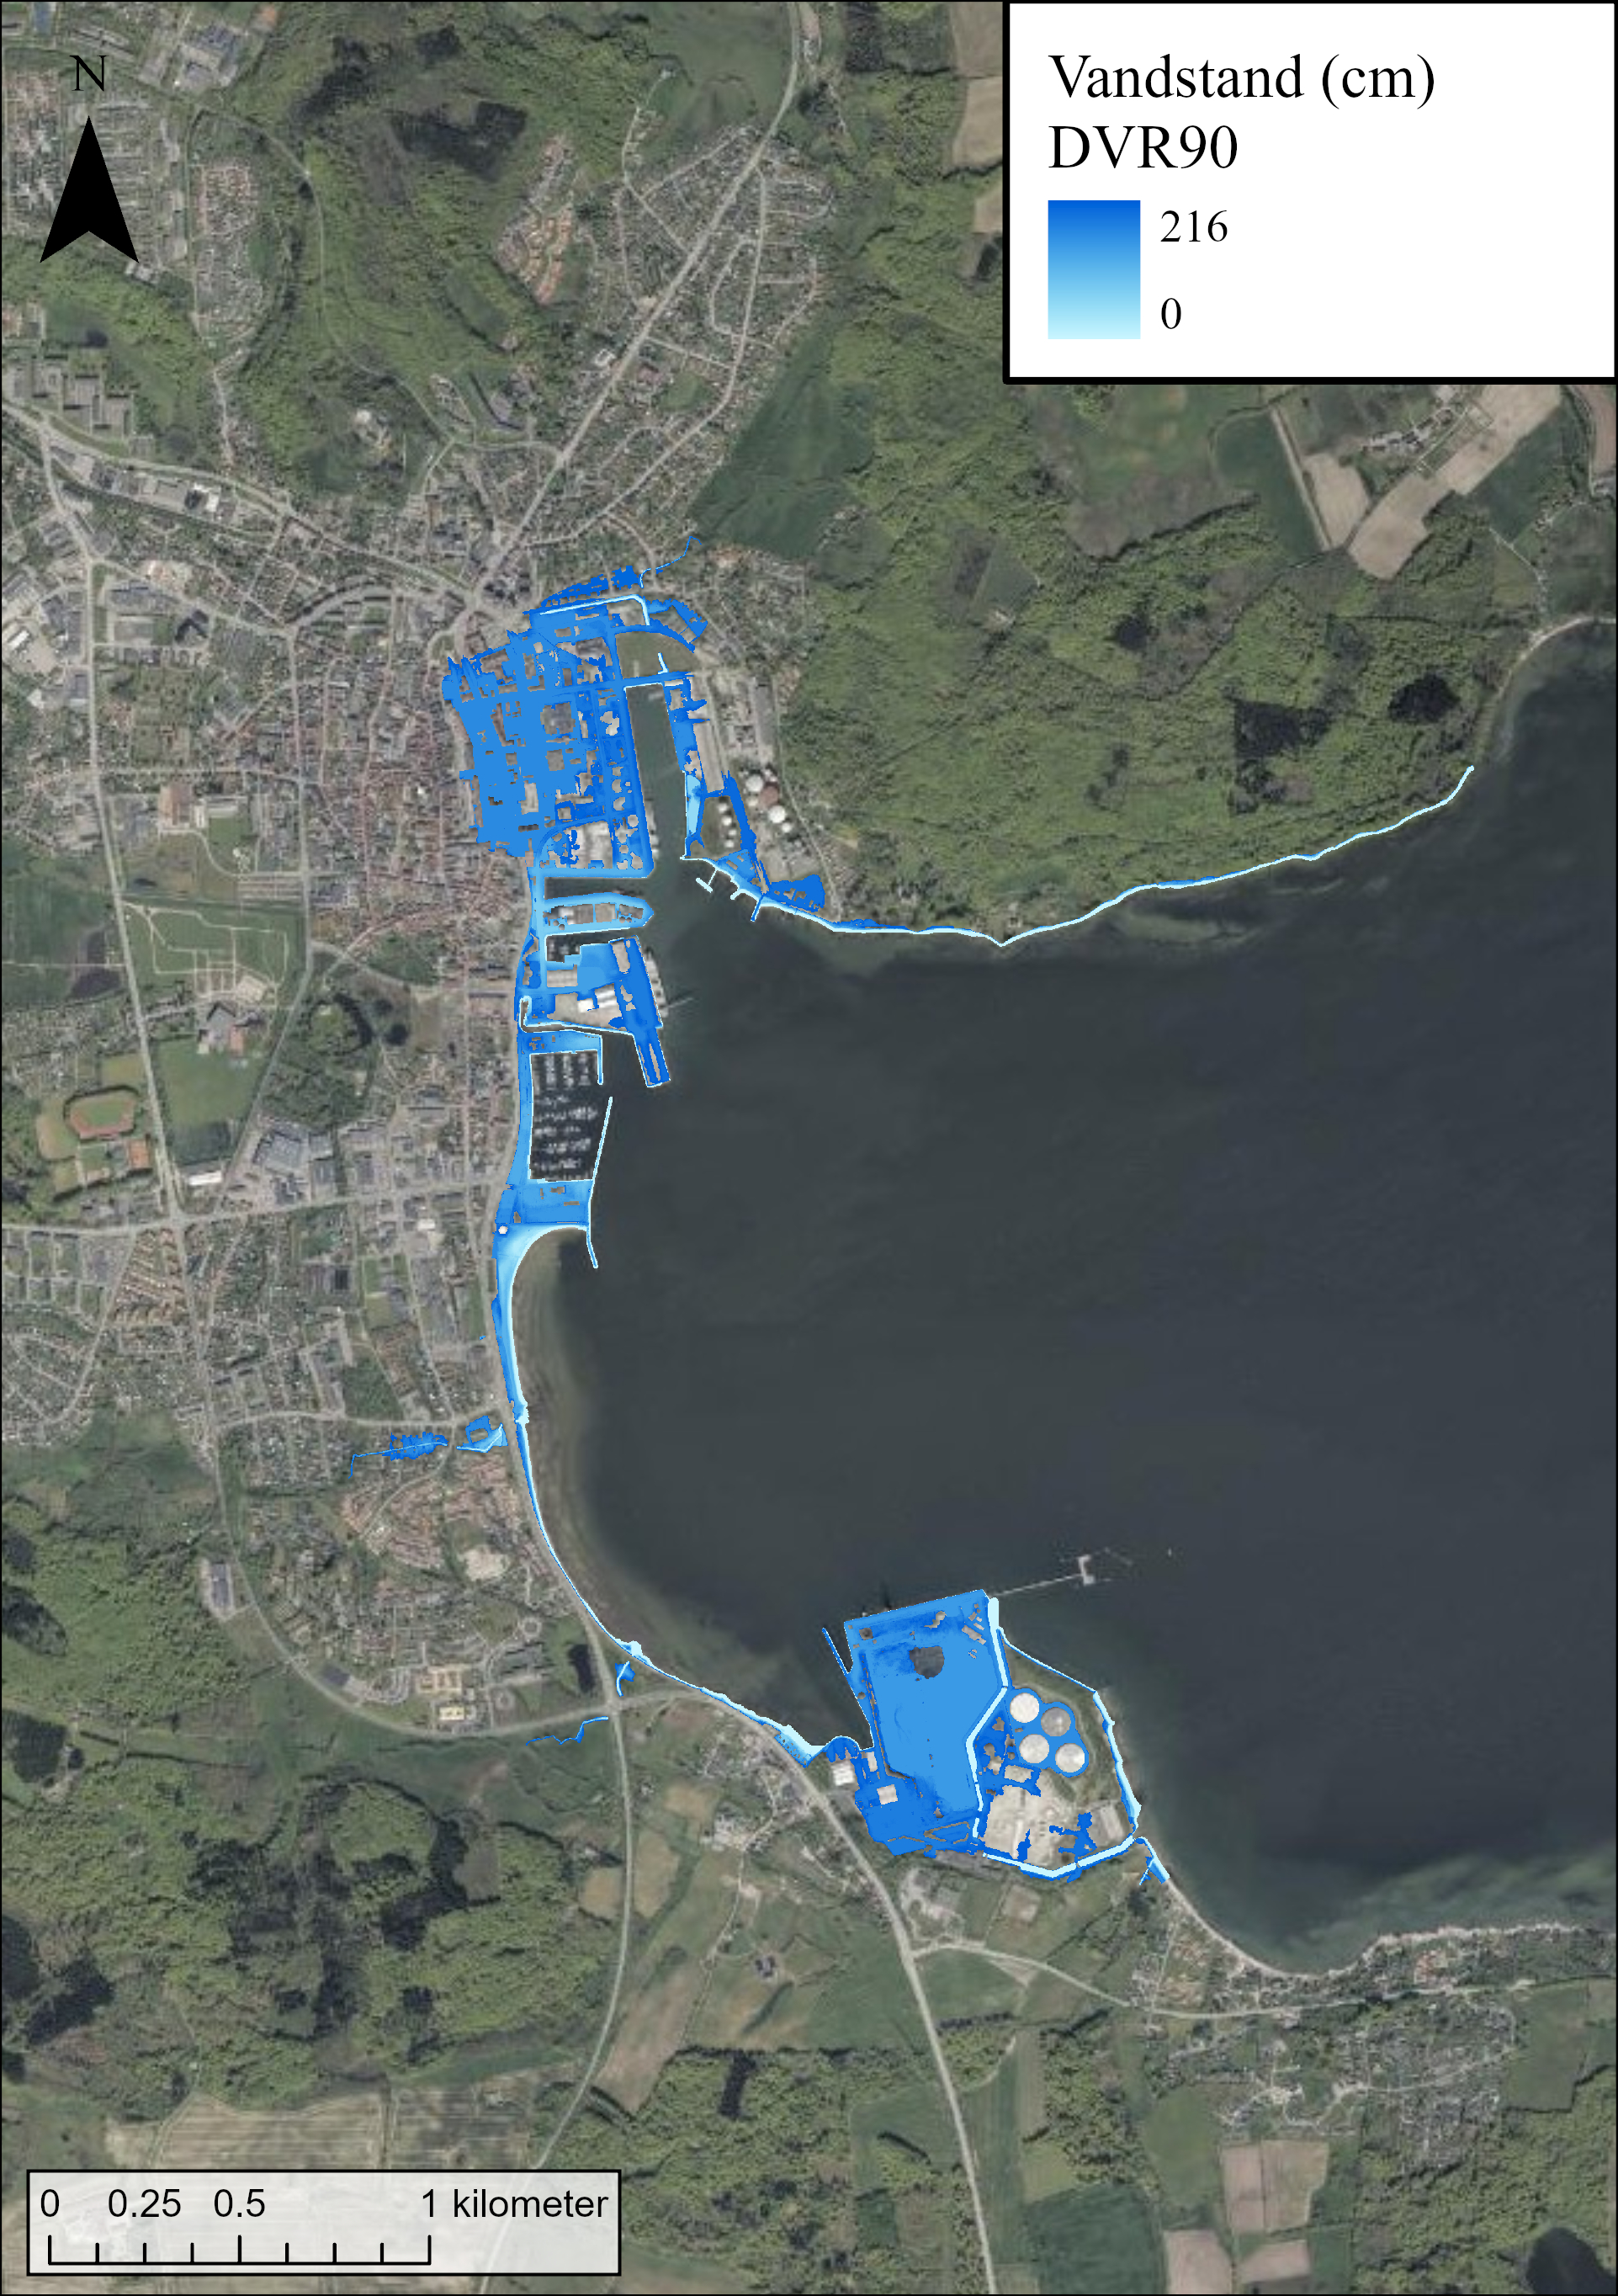
\includegraphics[width=0.8\linewidth]{images/Resultater/2023Malt/2023 resultat_aabenraa.jpg}
        \caption{Målte oversvømmelseskort over Aabenraa}
        \label{Subfig: Målt Aabenraa}
    \end{subfigure}
    \begin{subfigure}[t]{0.5\textwidth}
        \centering
        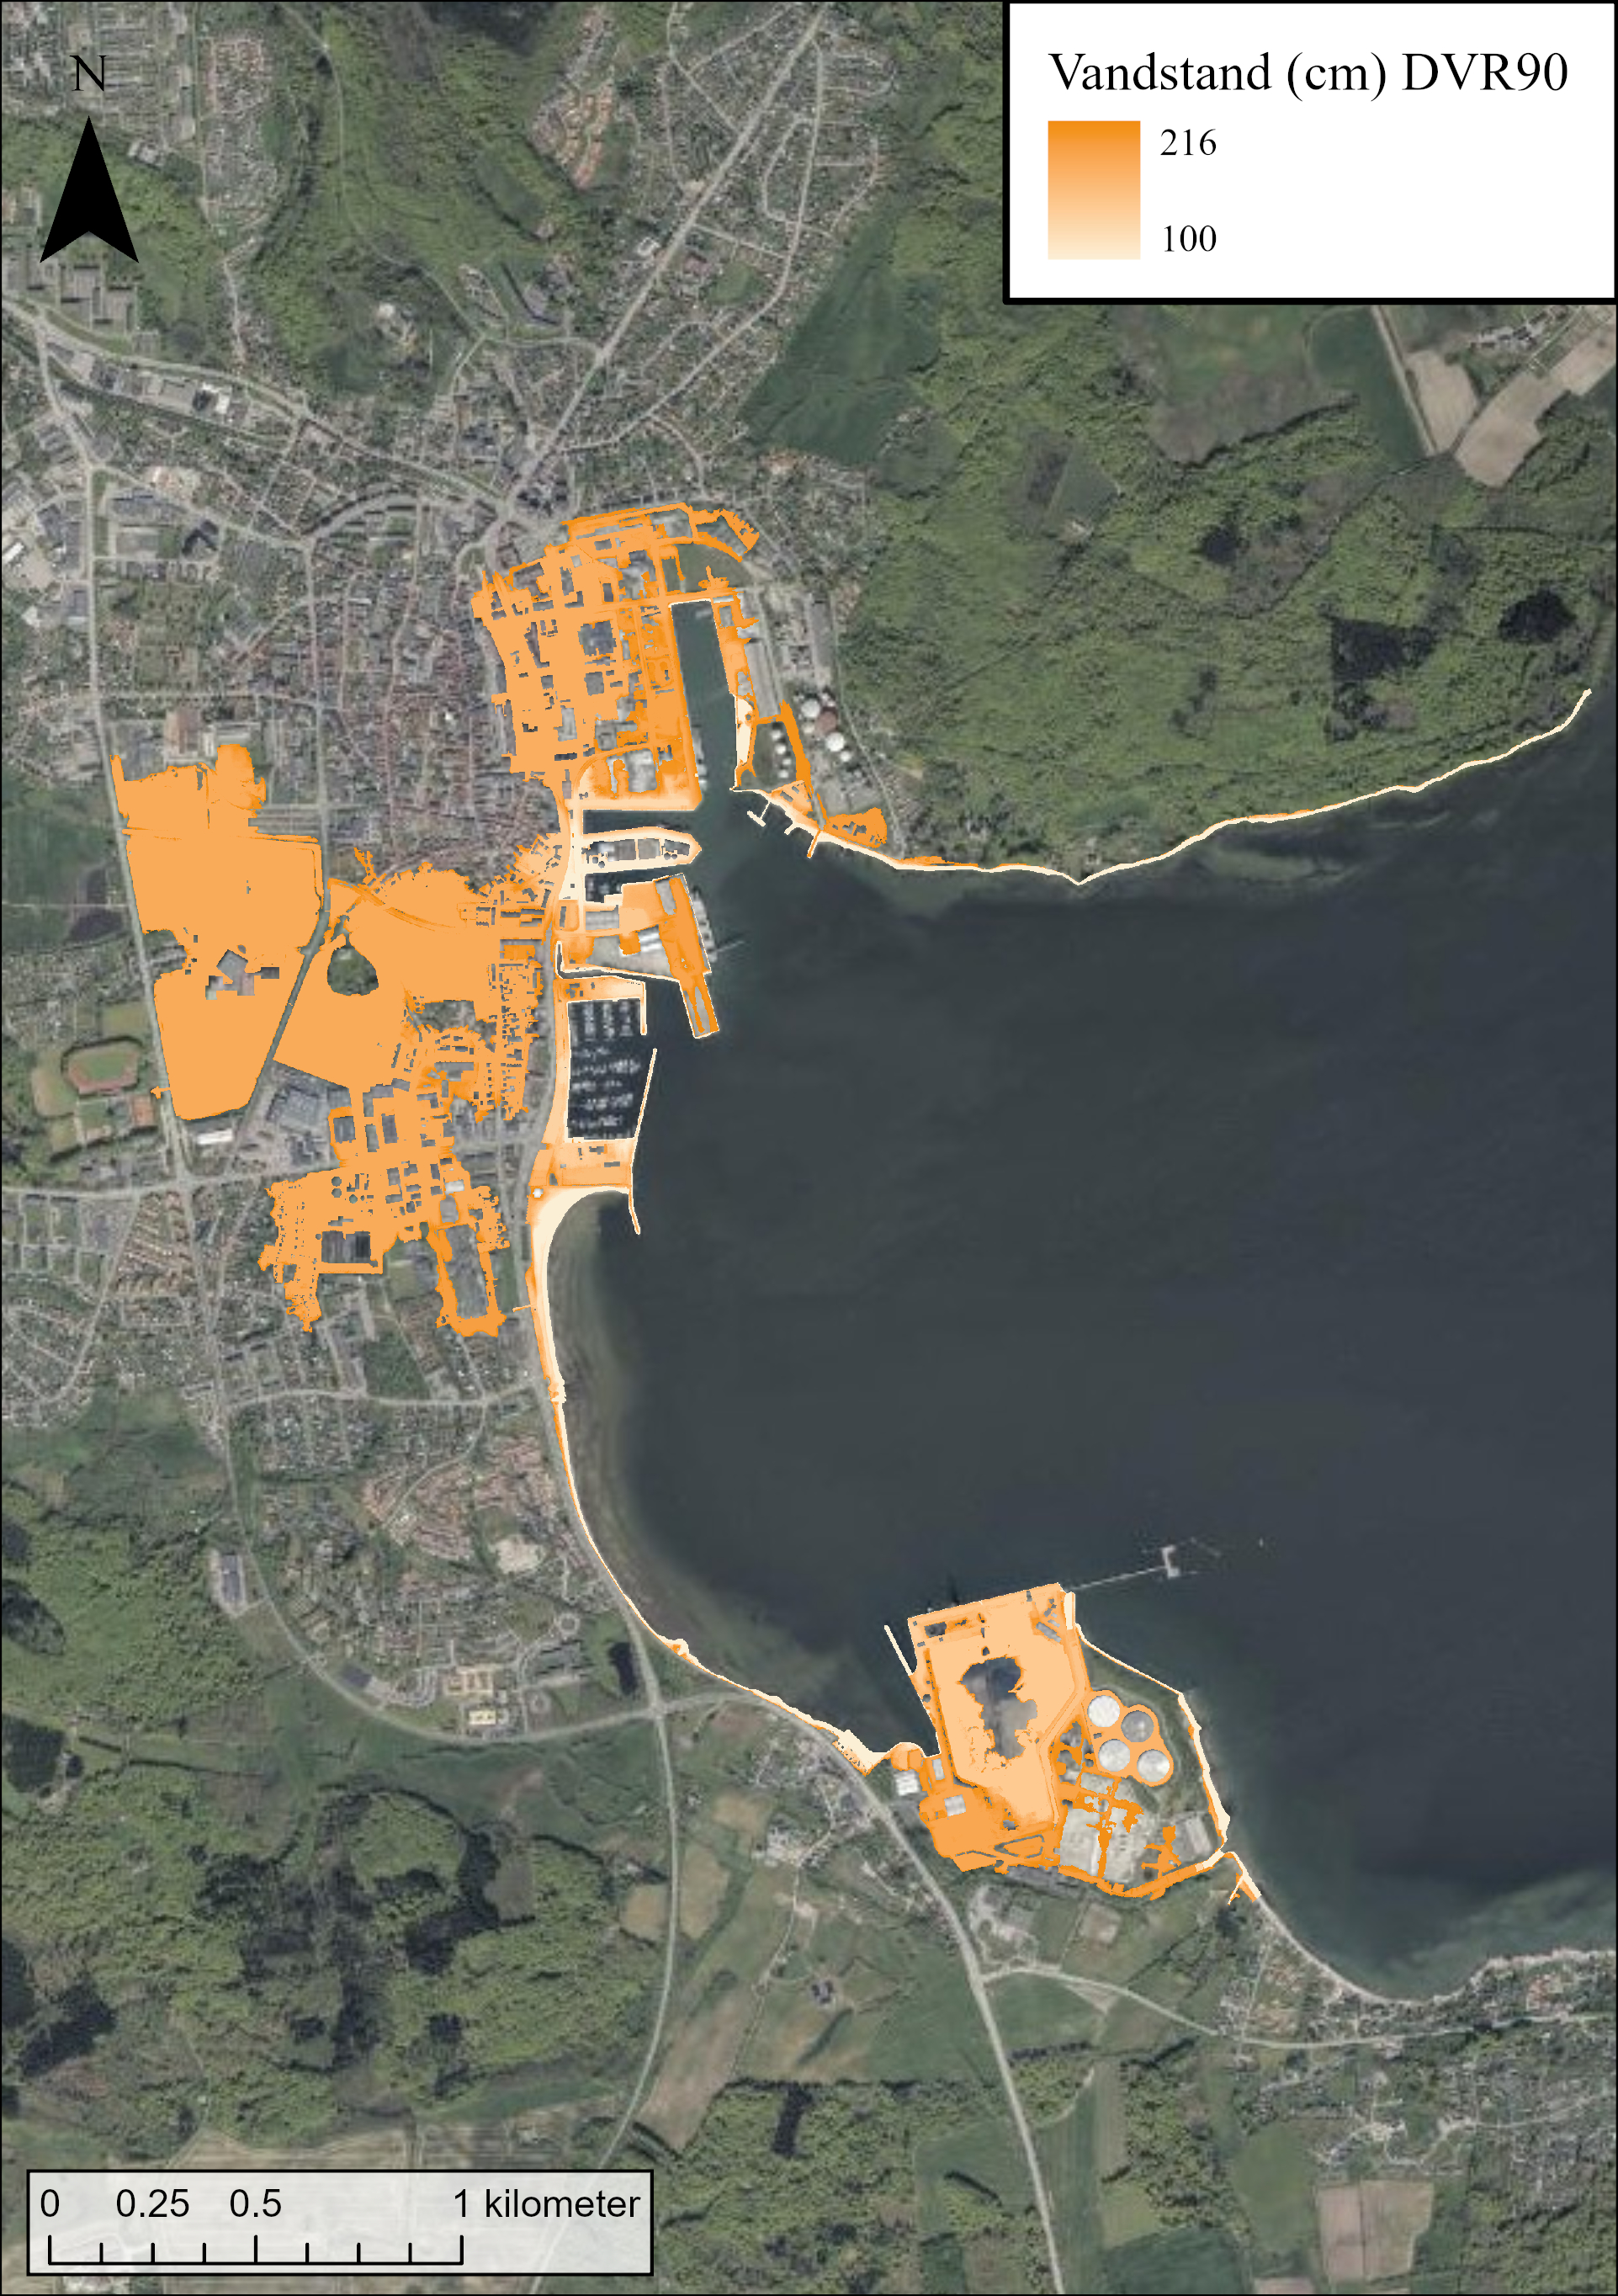
\includegraphics[width=0.8\linewidth]{images/Resultater/2023Model/2023 model_aabenraa.jpg}
        \caption{Simuleret oversvømmelseskort over Aabenraa}
        \label{Subfig: Model Aabenraa}
    \end{subfigure}
    \caption{Målt og simuleret oversvømmelseskort af oktober 2023 stormfloden for Aabenraa i centimeter over DVR90}
    \label{Figur: Målt & simuleret Aabenraa}
\end{figure}

Stormfloden i oktober 2023 i Aabenraa påvirkede syv forskellige arealanvendelser. I figur \ref{Figur: Påvirket arealanvendelse Aabenraa} er der vist hvor hvilke arealer der blev påvirket under den målte stormflod og den simuleret som procent af det totale oversvømmet areal. For den målte hændelse var de mest påvirkede områder de bebyggede områder med 41,8\%, erhverv med 25\% og infrastruktur med 23\%. \\
Resultatet fra modellen har ligeledes lignende påvirkede områder med 28,7\% bebyggede områder, 20,6\% erhverv og 21,5\% infrastruktur. Dertil er der stor forskel mellem målt og simulerede resultat ved rekreativt areal hvor 0,6\% blev oversvømmet ved den målte hændelse og 19,5\% oversvømmet ved det simulerede resultat. 

\begin{figure}[H]
    \centering
    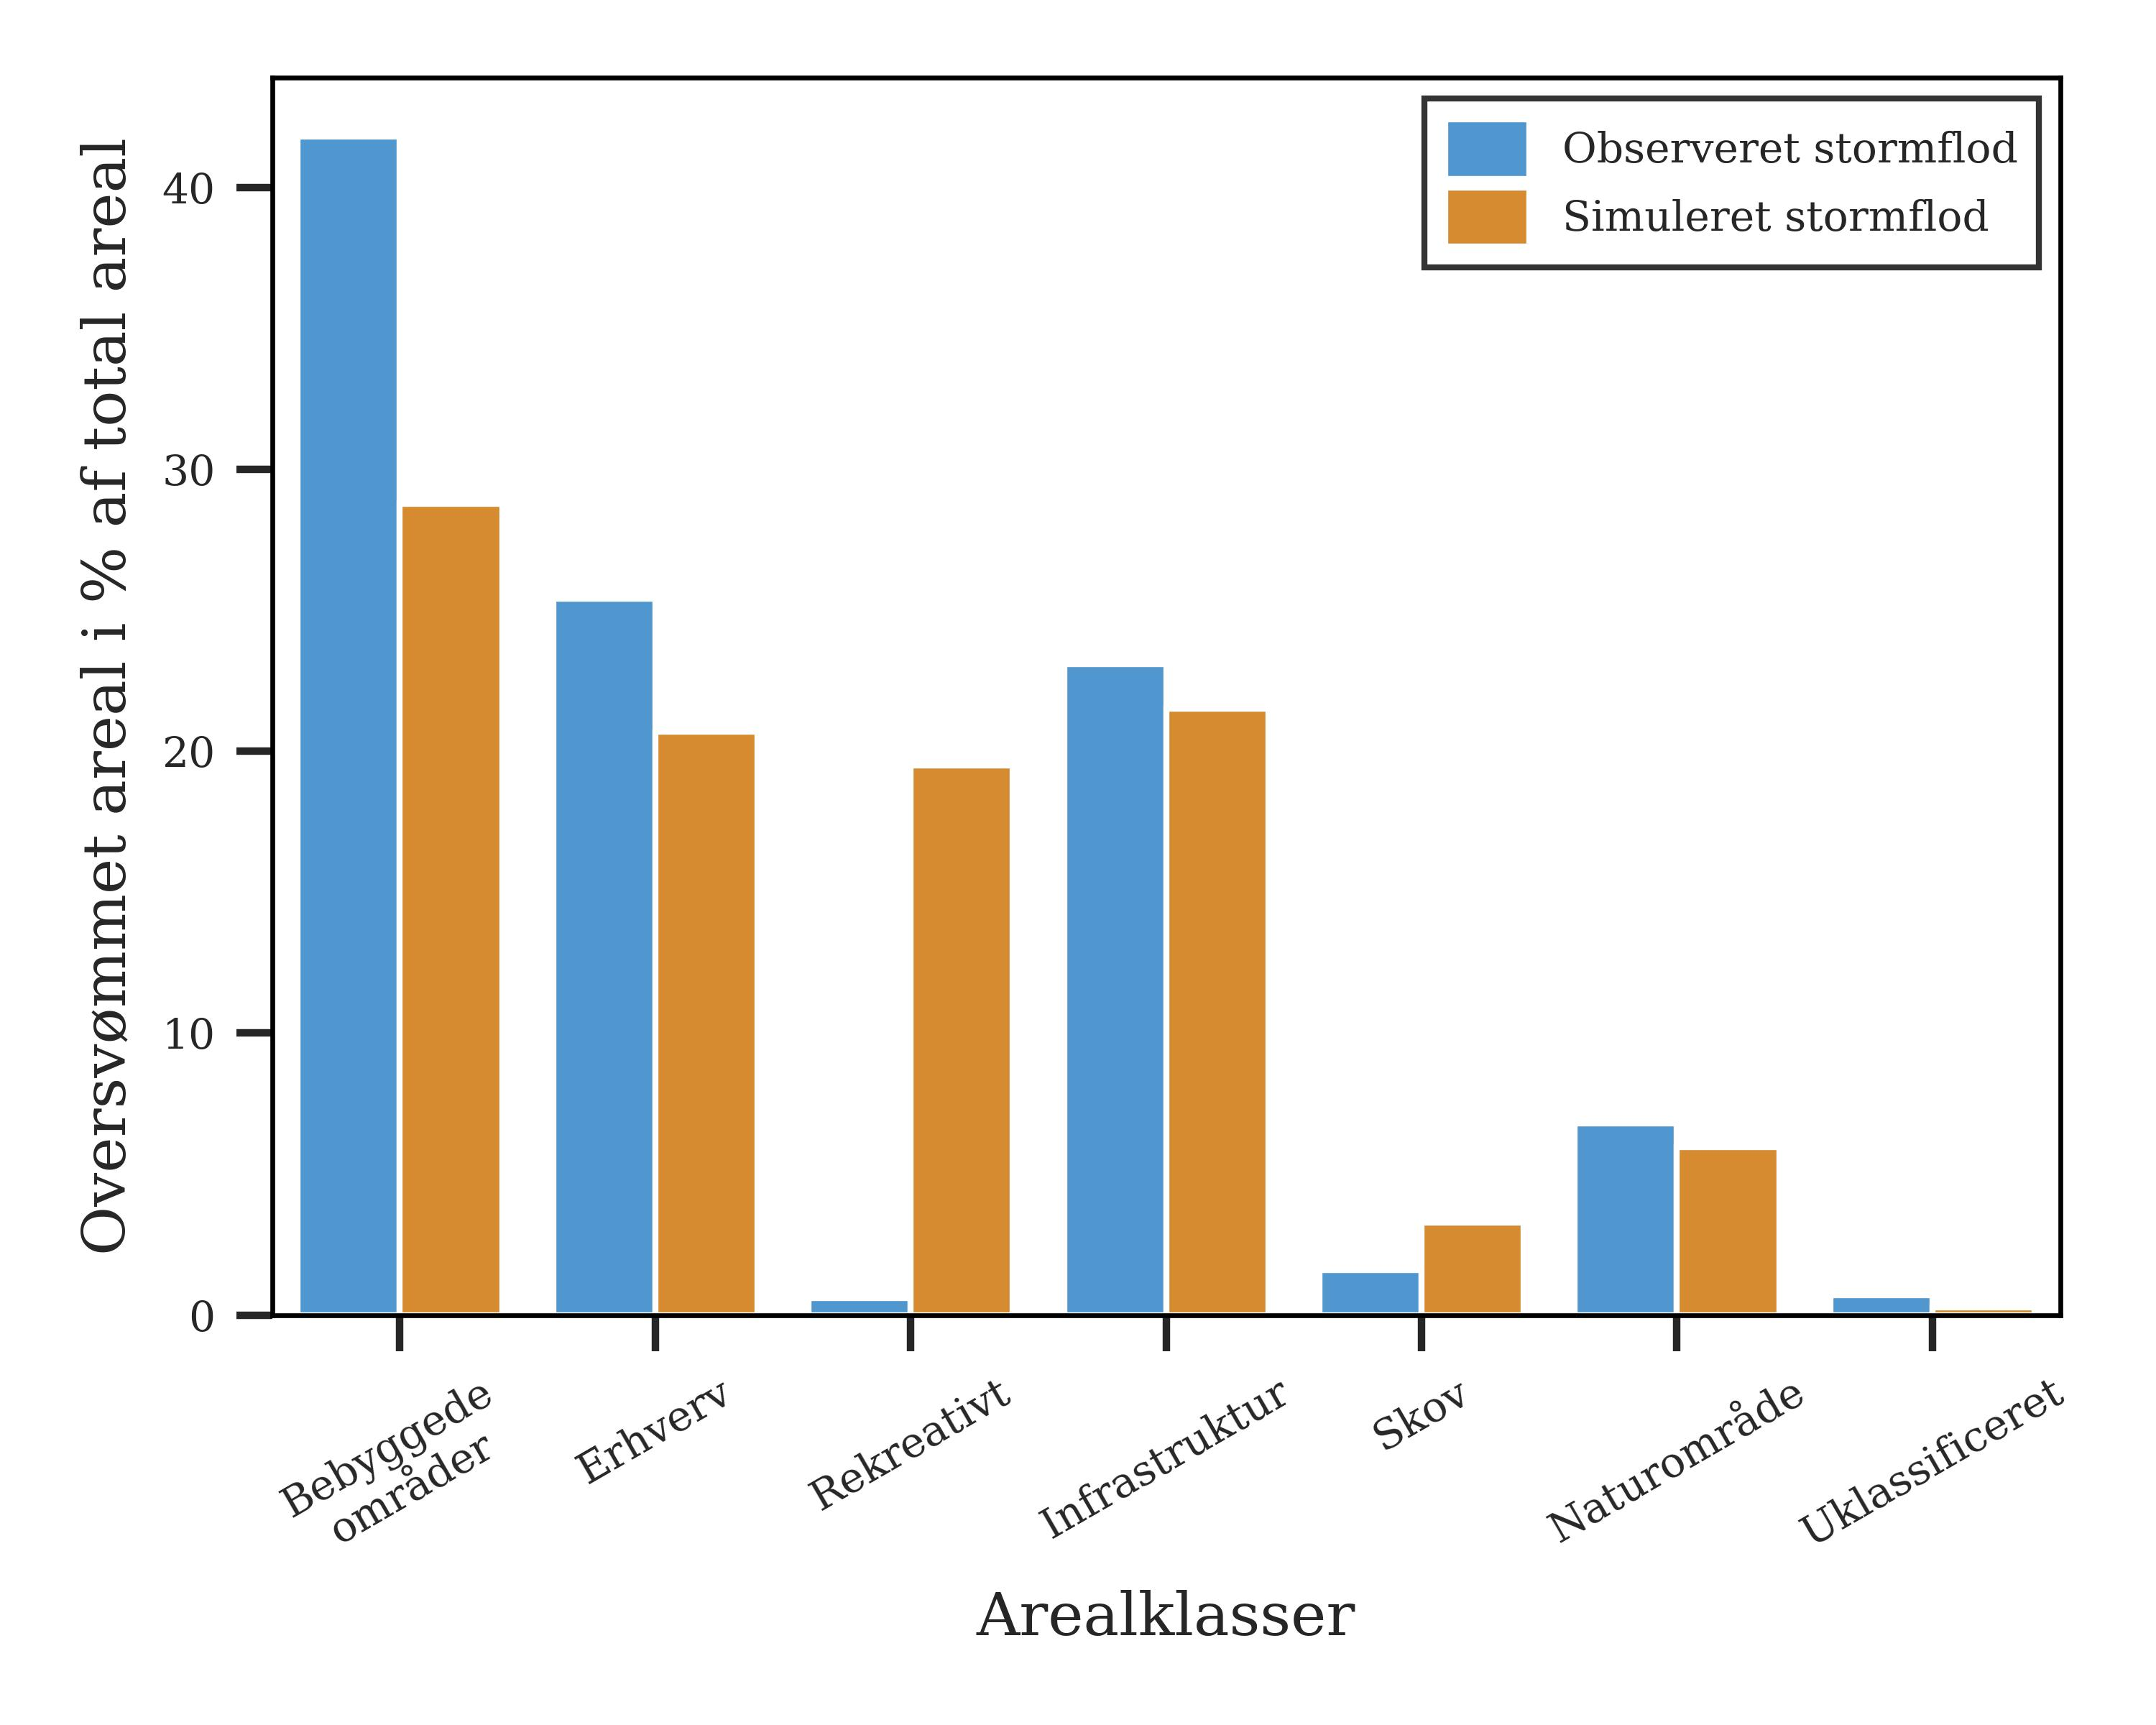
\includegraphics[width=0.8\linewidth]{images/Resultater/areal_anvendelses_grafer/aabenraa_arealanvendelse.jpg}
    \caption{Påvirkede arealanvendelsesklasser som procent af totalt oversvømmet areal i Aabenraa for den målte og simuleret oktober 2023 stormflods hændelse}
    \label{Figur: Påvirket arealanvendelse Aabenraa}
\end{figure}

I figur \ref{Subfig: Målt Gedser} er den målte oversvømmelse af Gedser Havn af oktober 2023 stormfloden. I figur \ref{Subfig: Model Gedser} er det simulerede resultat. Resultatet fra Inundation Modellen er meget ens til den målte hændelse. Den målte hændelse havde et oversvømmet areal på 344735 m\textsuperscript{2} kontra 331875 m\textsuperscript{2} fra Inundation Modellen. Dette er en forskel på 3,76\% svarende til 12969 m\textsuperscript{2}.  

\begin{figure}[H]
    \begin{subfigure}[t]{0.5\textwidth}
        \centering
        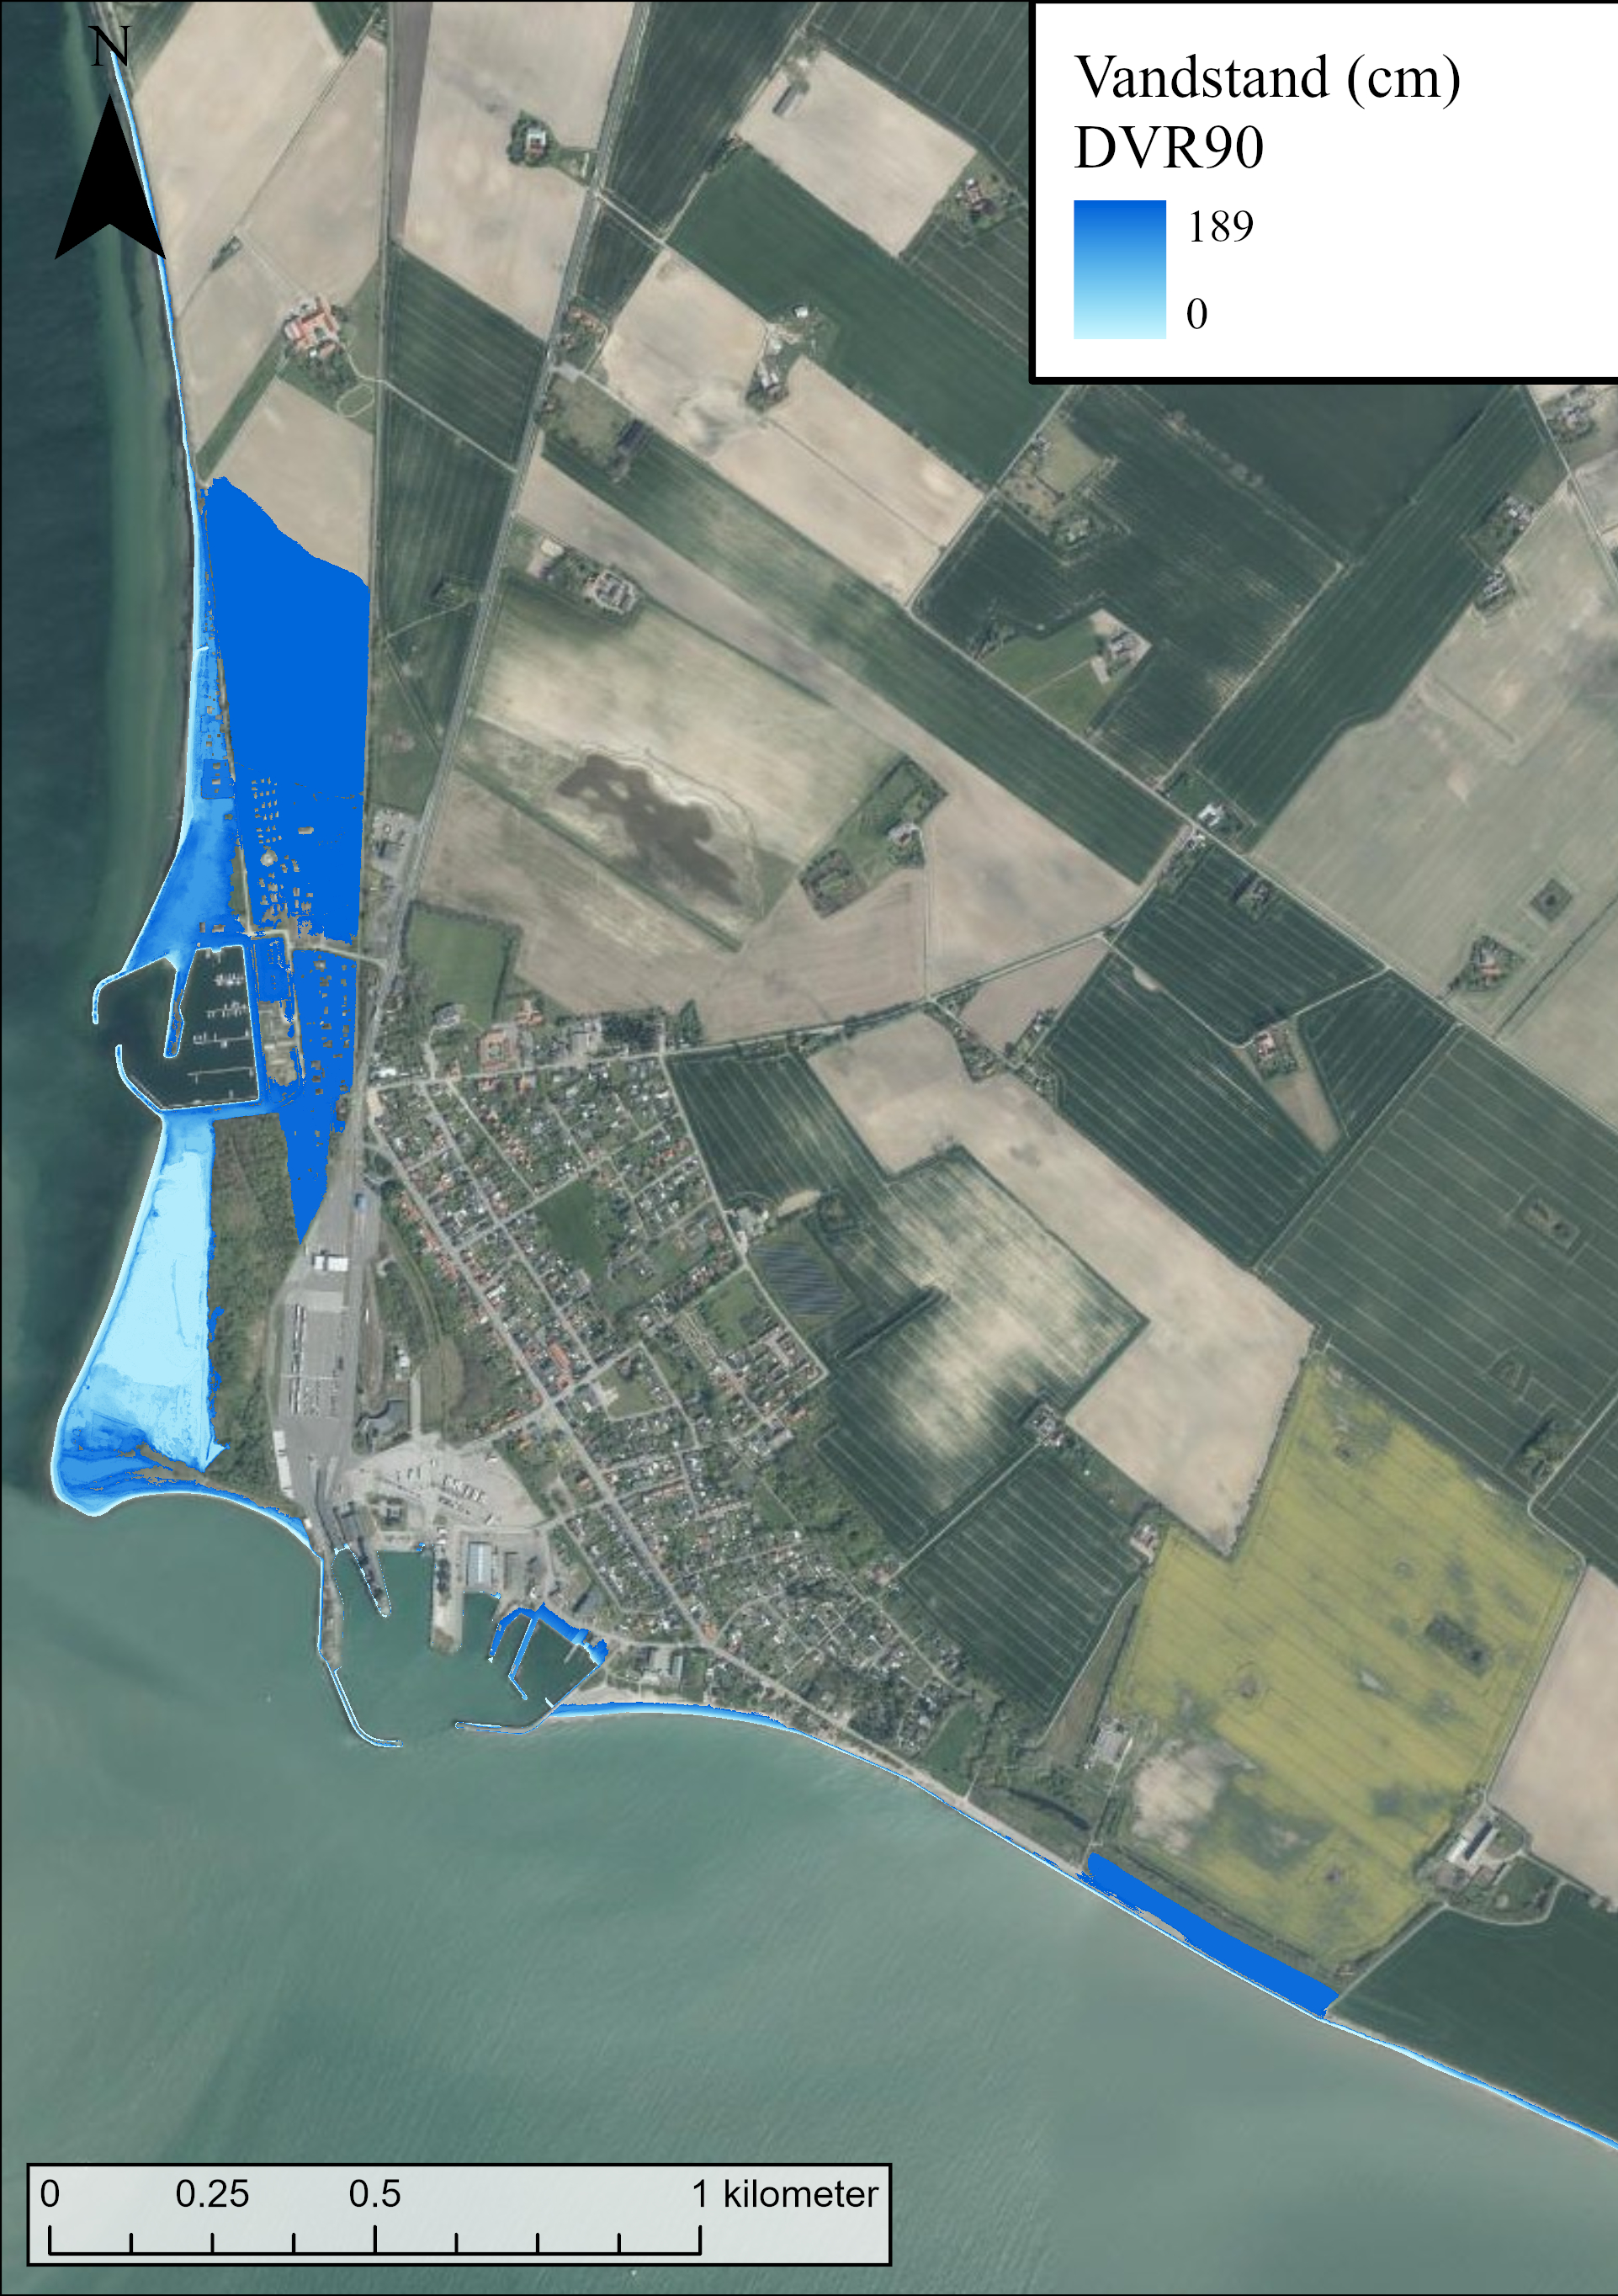
\includegraphics[width=0.8\linewidth]{images/Resultater/2023Malt/2023 resultat_gedser.jpg}
        \caption{Målte oversvømmelseskort over Gedser Havn}
        \label{Subfig: Målt Gedser}
    \end{subfigure}
    \begin{subfigure}[t]{0.5\textwidth}
        \centering
        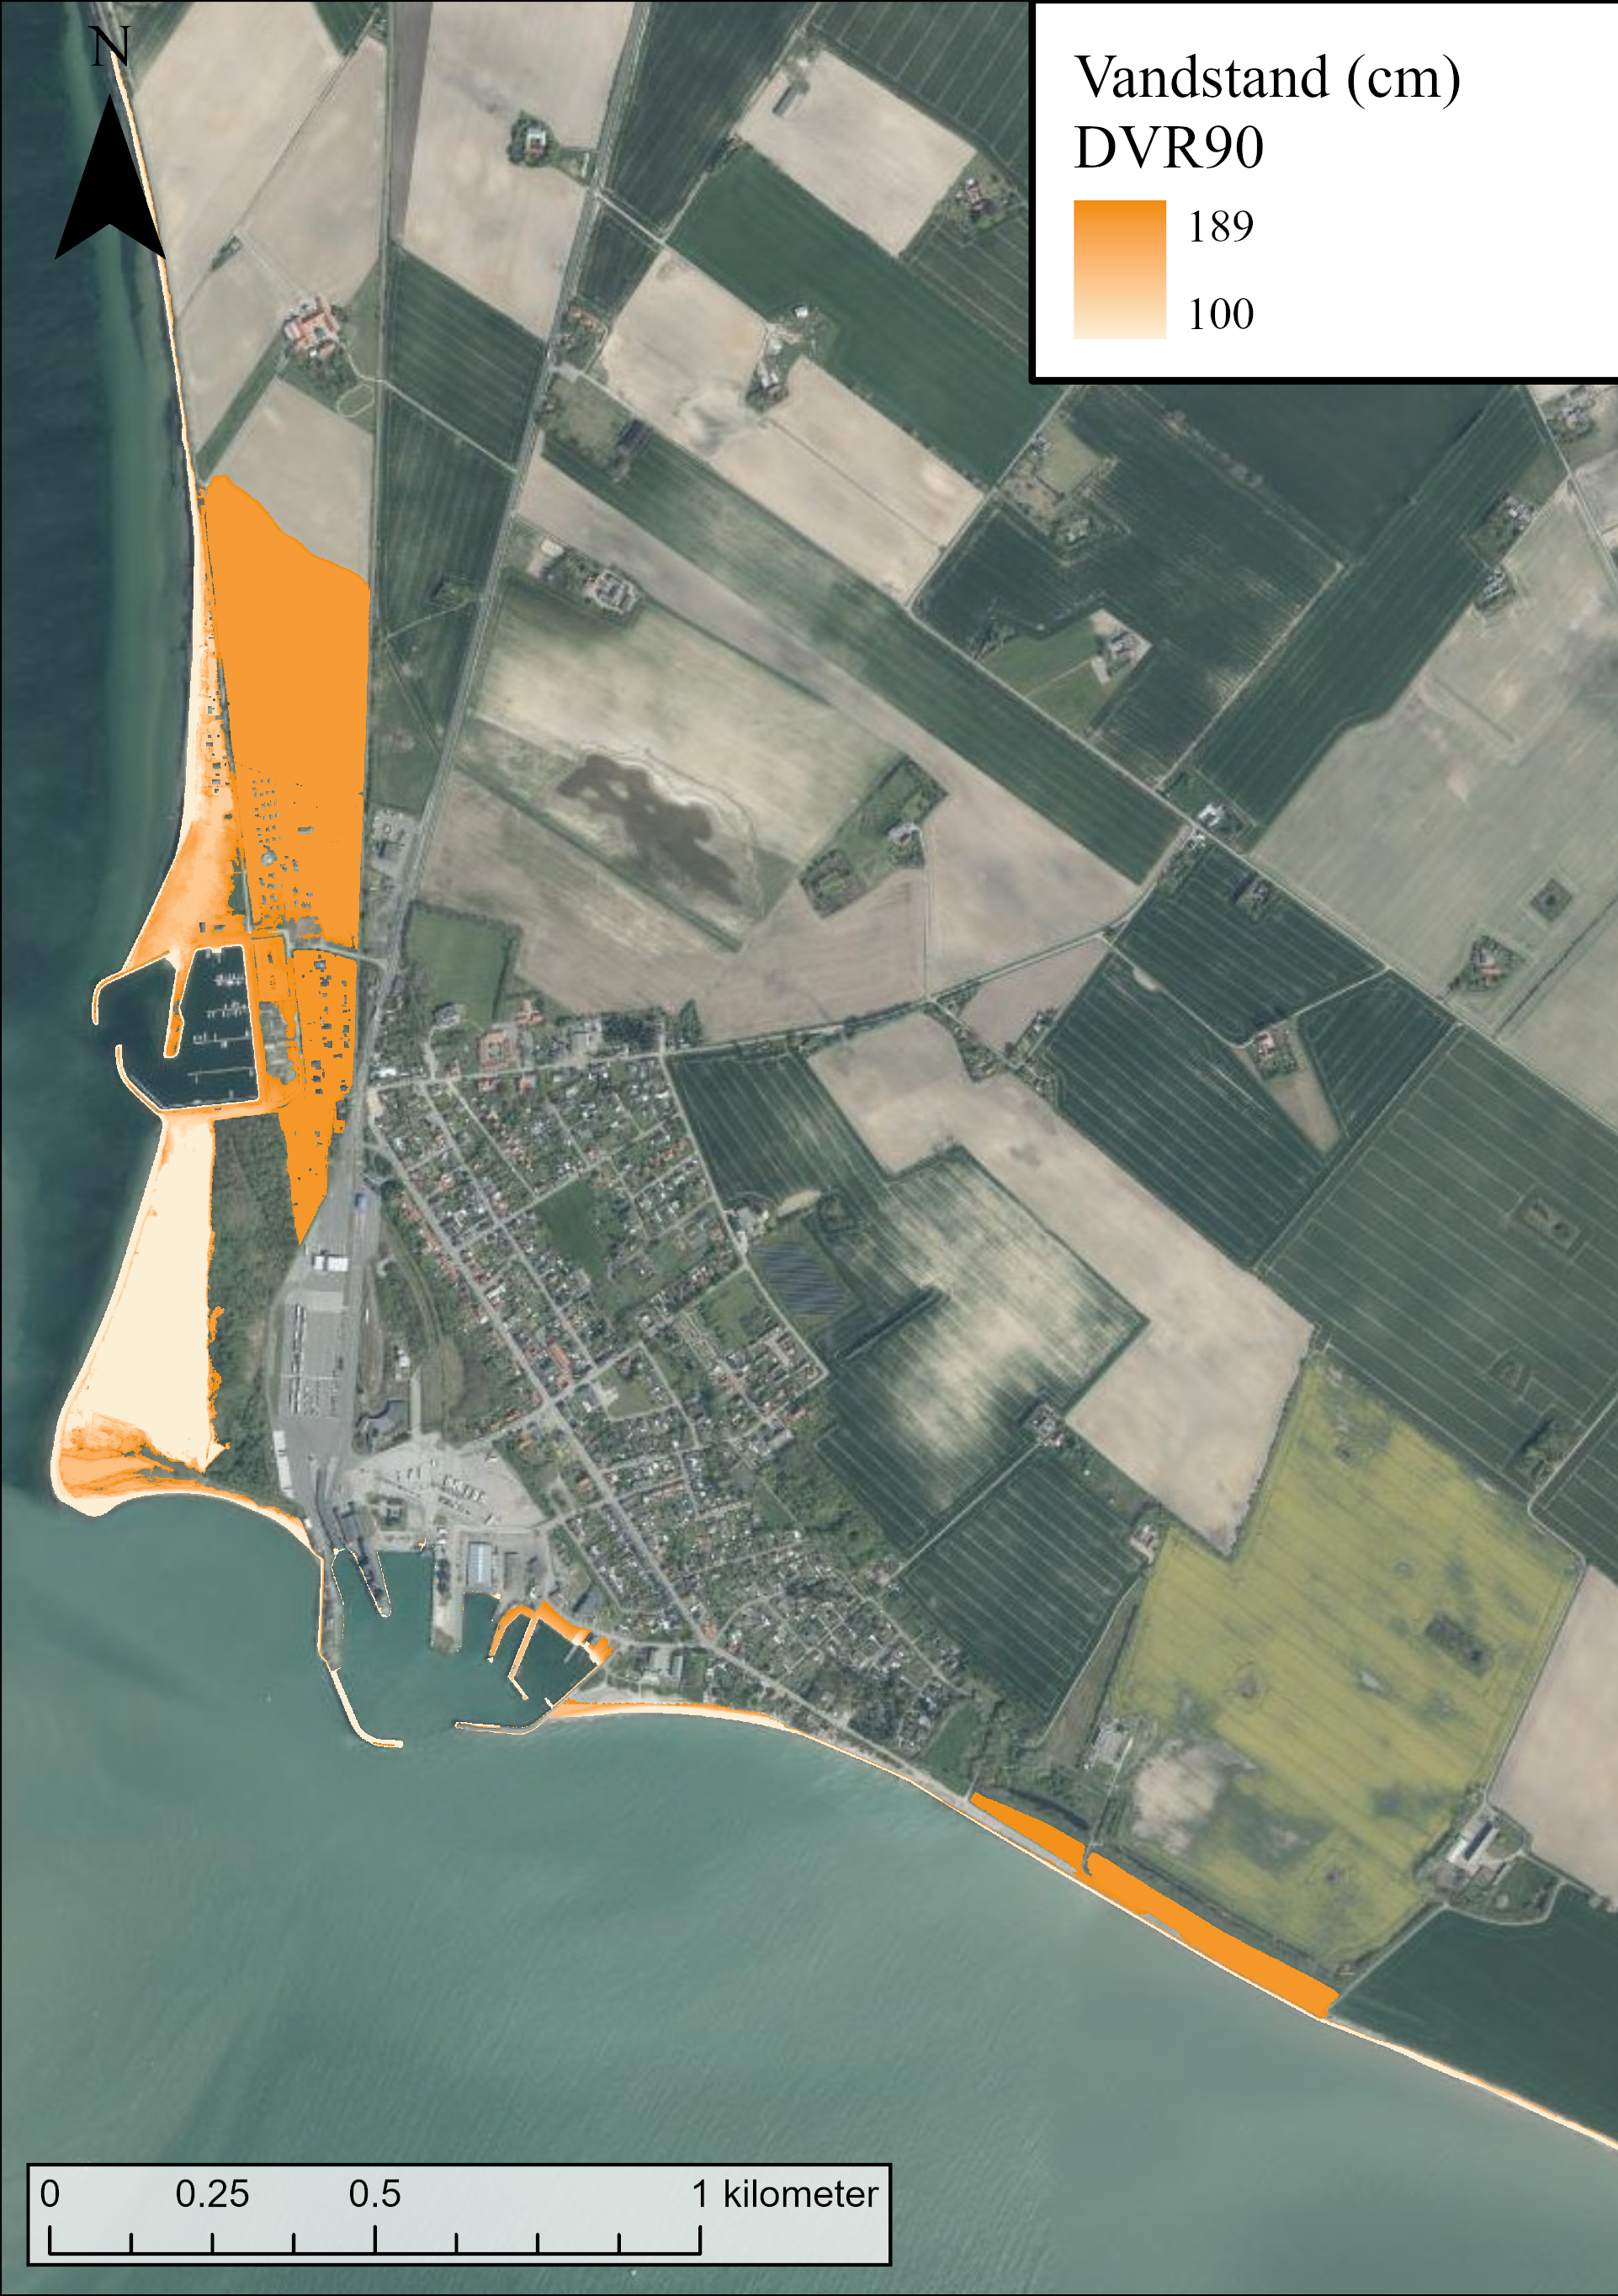
\includegraphics[width=0.8\linewidth]{images/Resultater/2023Model/2023 model_gedser.jpg}
        \caption{Simuleret oversvømmelseskort over Gedser Havn}
        \label{Subfig: Model Gedser}
    \end{subfigure}
    \caption{Målt og simuleret oversvømmelseskort af oktober 2023 stormfloden for Gedser Havn i centimeter over DVR90}
    \label{Figur: Målt & simuleret Gedser}
\end{figure}

I Gedser Havn blev otte arealklasser påvirket af oversvømmelserne under stormfloden i oktober 2023. Ved både den målte og simuleret stormflod er det naturområder der blev mest påvirket med henholdsvis 51,5 og 51,7\%. Andre arealer påvirket indebærer landbrug med 12,2 og 12,5\%, infrastruktur med 11,4 og 10,8\% og bebyggede områder med 10,9\% for begge (figur \ref{Figur: Påvirket arealanvendelse Gedser}).

\begin{figure}[H]
    \centering
    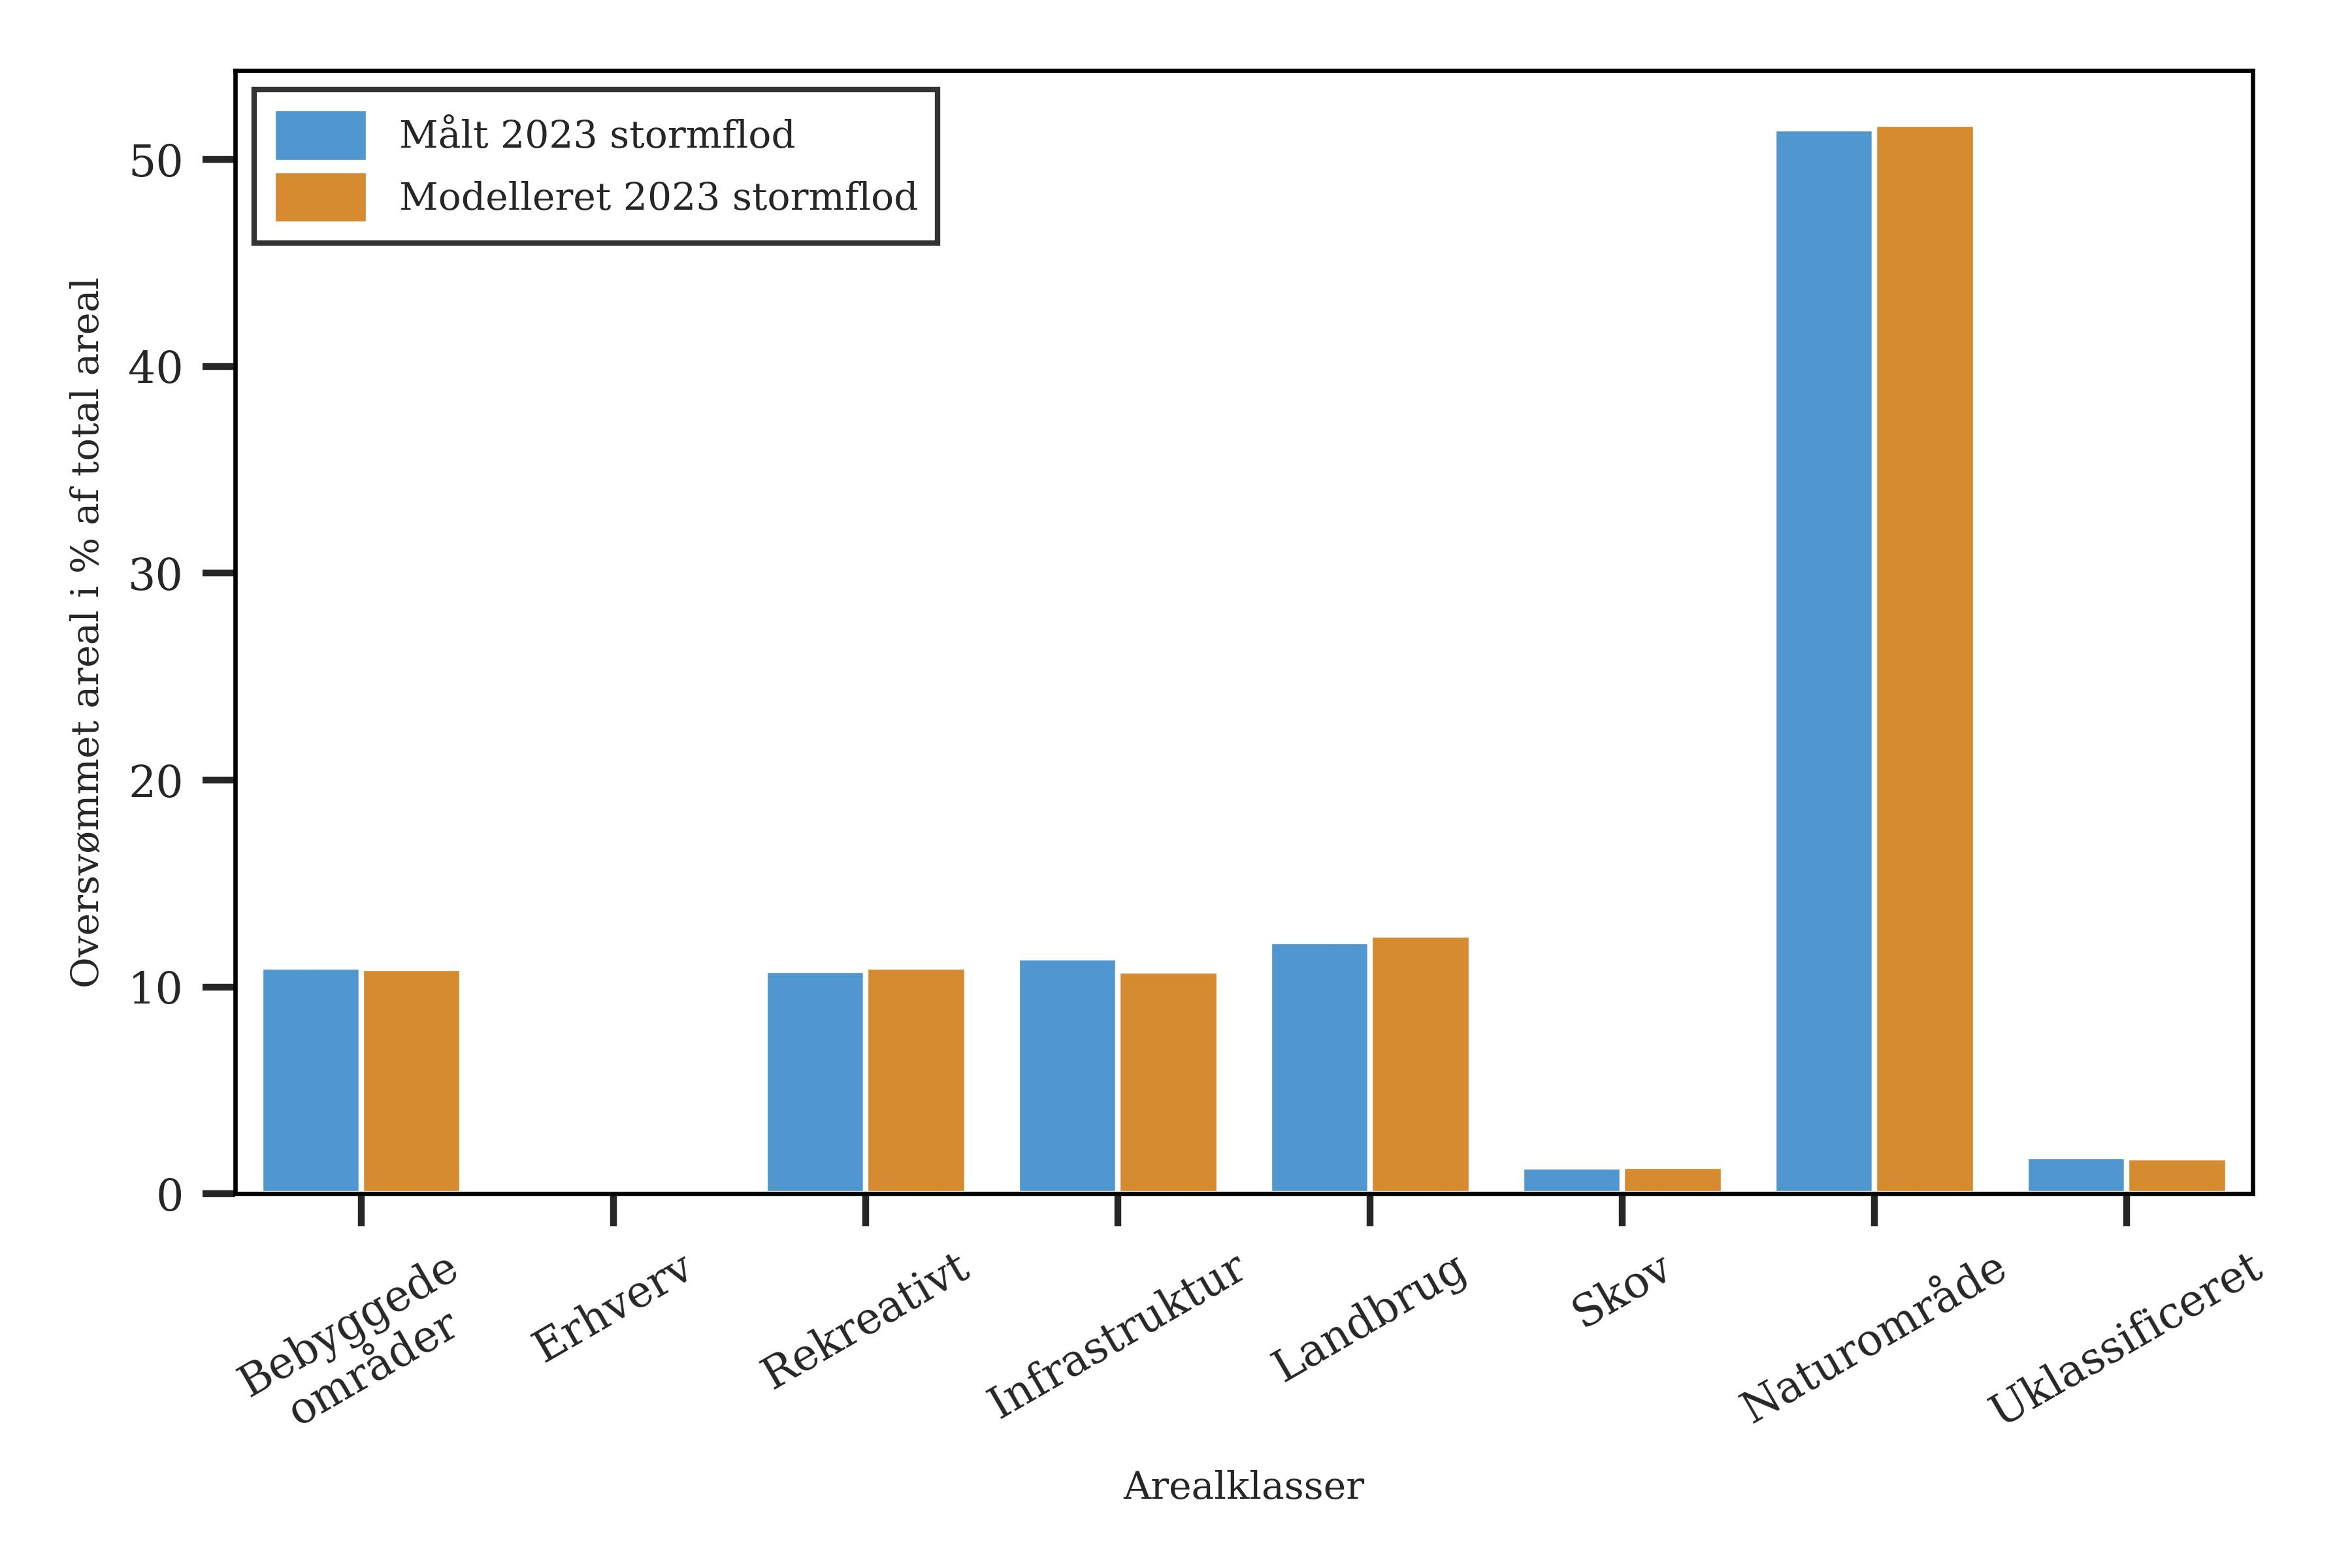
\includegraphics[width=0.8\linewidth]{images/Resultater/areal_anvendelses_grafer/gedser_arealanvendelse.jpg}
    \caption{Påvirkede arealanvendelsesklasser som procent af totalt oversvømmet areal i Gedser Havn for den målte og simuleret oktober 2023 stormflods hændelse}
    \label{Figur: Påvirket arealanvendelse Gedser}
\end{figure}

For Hesnæs var det primært havnen og kystlinjen der blev oversvømmet under stormfloden i 2023 (figur \ref{Subfig: Målt Hesnæs}). Resultatet fra Inundation Modellen i figur \ref{Subfig: Model Hesnæs} giver det samme resultat og der er ikke stor forskel mellem målt hændelse og simuleret resultat. Den målte hændelse havde et totalt oversvømmet areal på 34572 m\textsuperscript{2} og det simulerede resultat havde et areal på 32780 m\textsuperscript{2}. Modellens resultat er derfor 1791 m\textsuperscript{2} mindre, svarende til en forskel på 5,2\%.  

\begin{figure}[H]
    \begin{subfigure}[t]{0.5\textwidth}
        \centering
        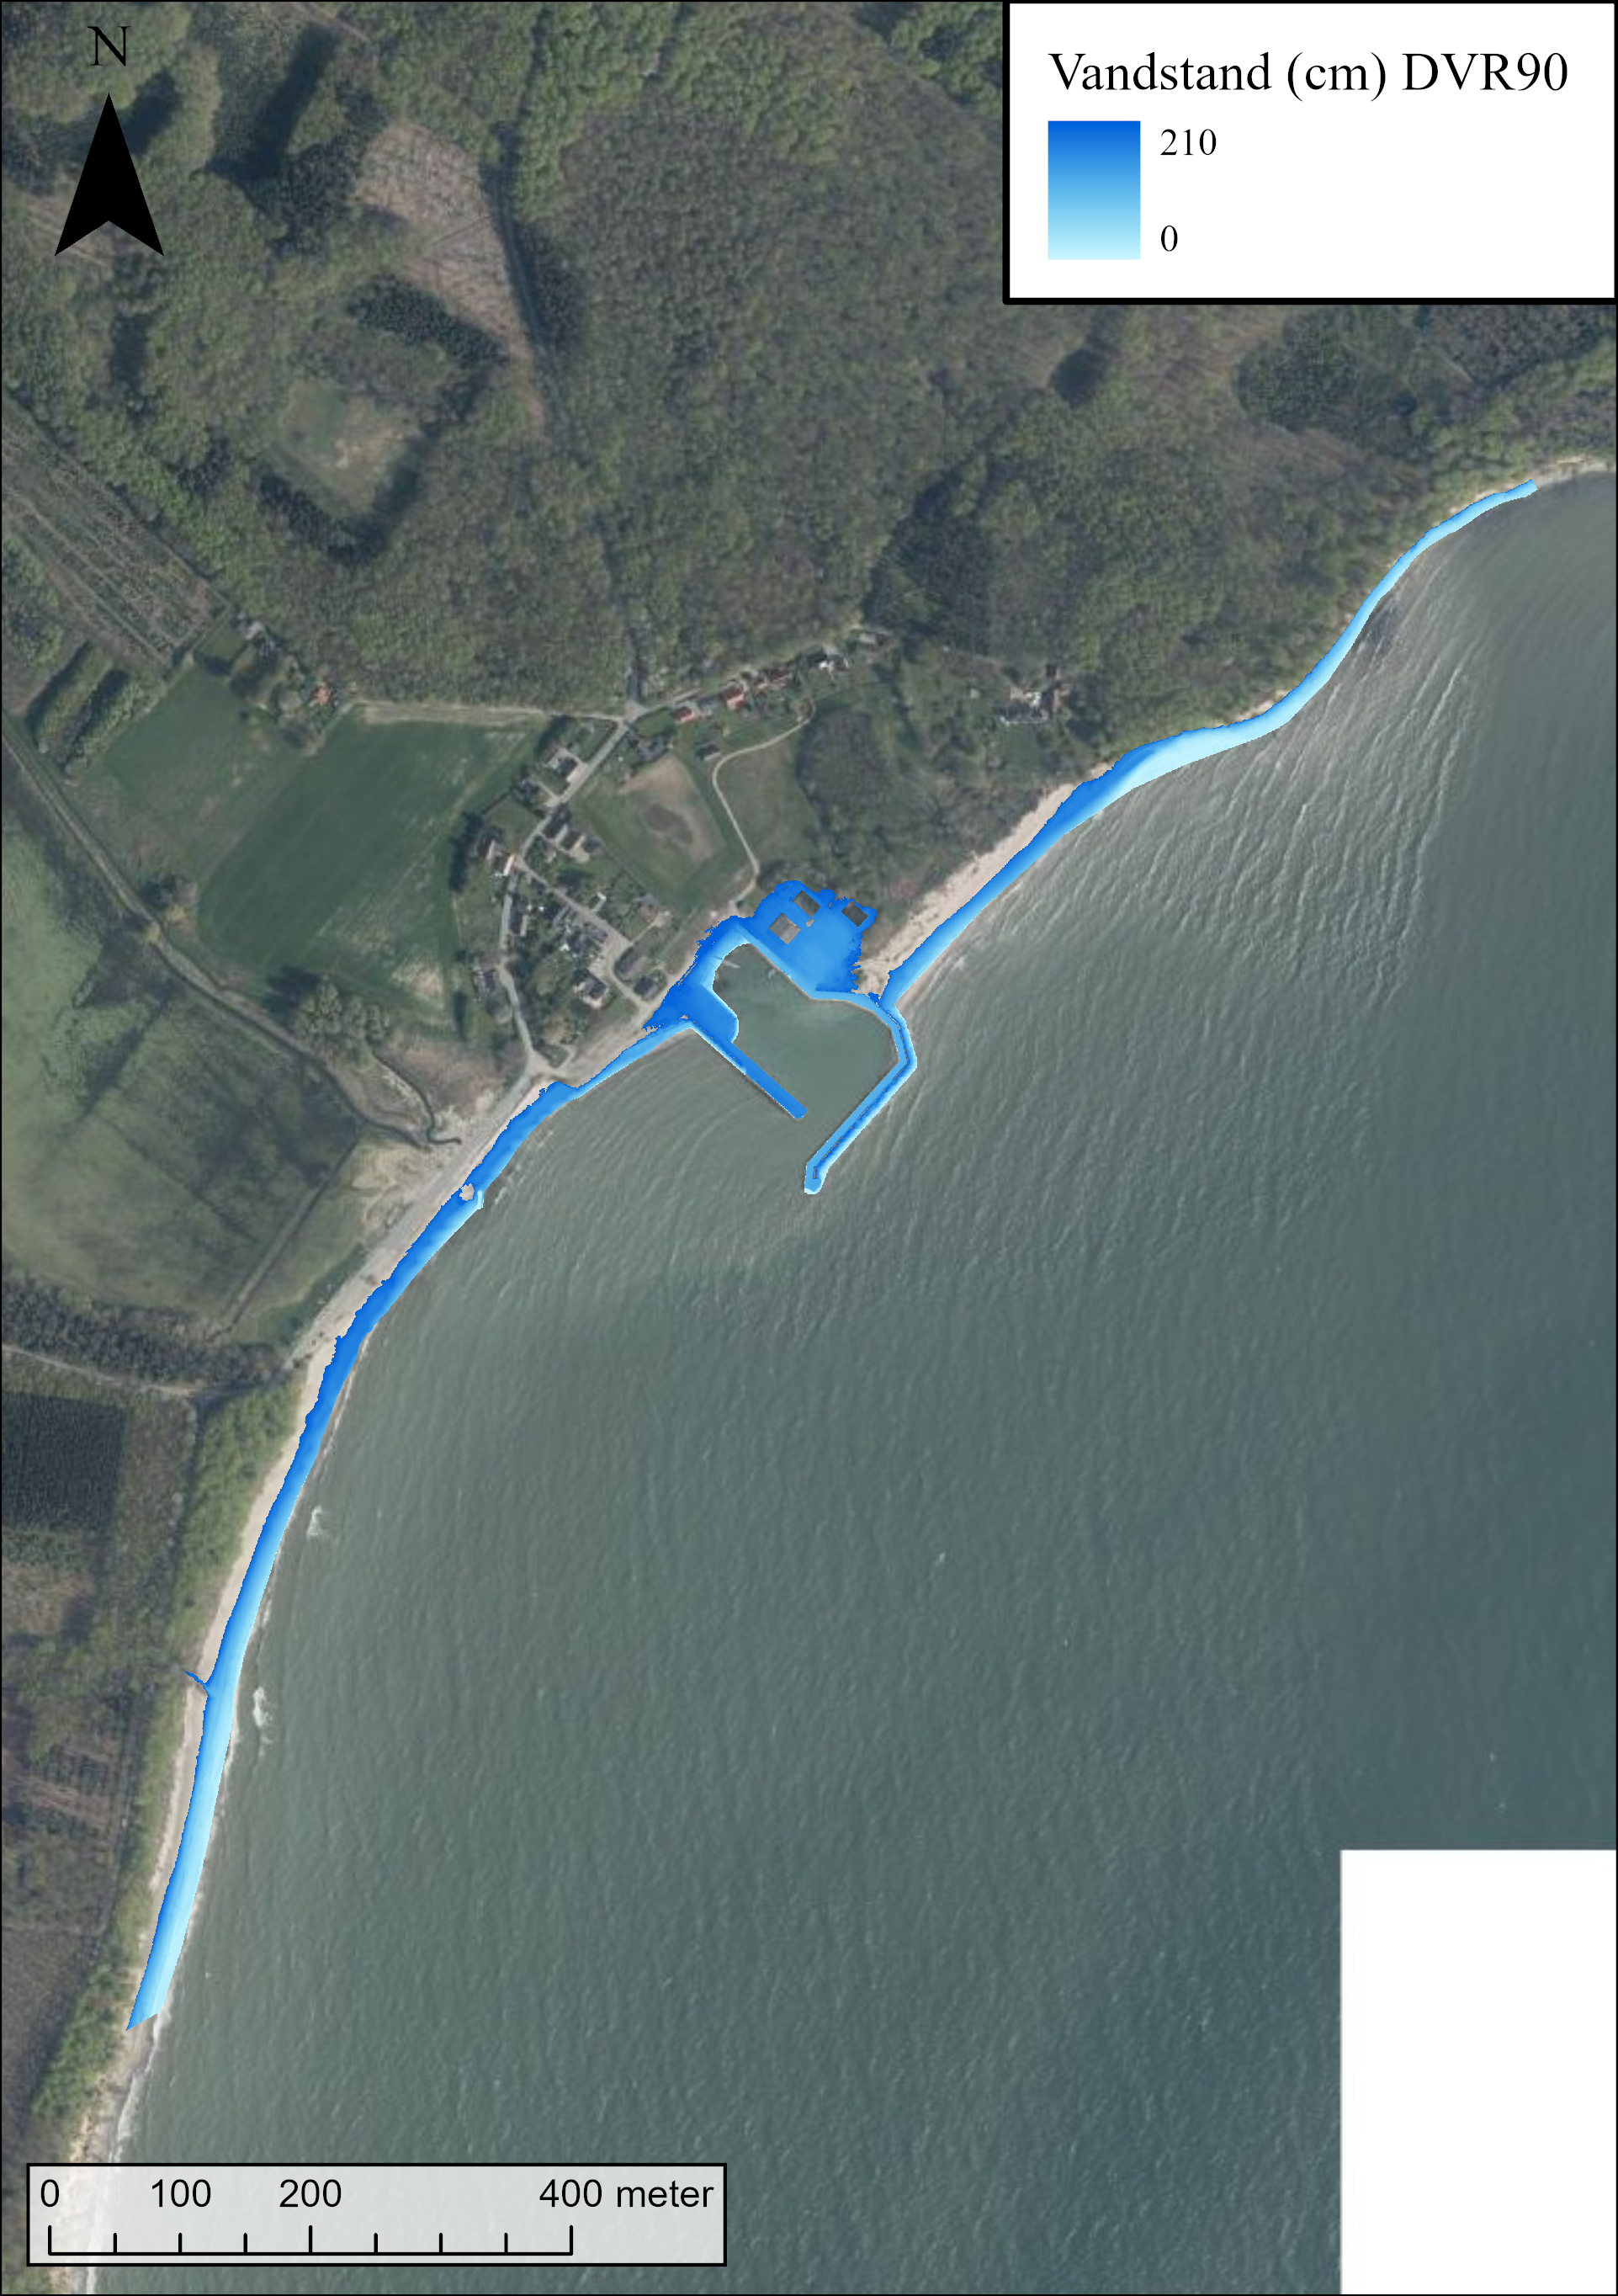
\includegraphics[width=0.8\linewidth]{images/Resultater/2023Malt/2023 resultat_hesnaes.jpg}
        \caption{Målte oversvømmelseskort over Hesnæs}
        \label{Subfig: Målt Hesnæs}
    \end{subfigure}
    \begin{subfigure}[t]{0.5\textwidth}
        \centering
        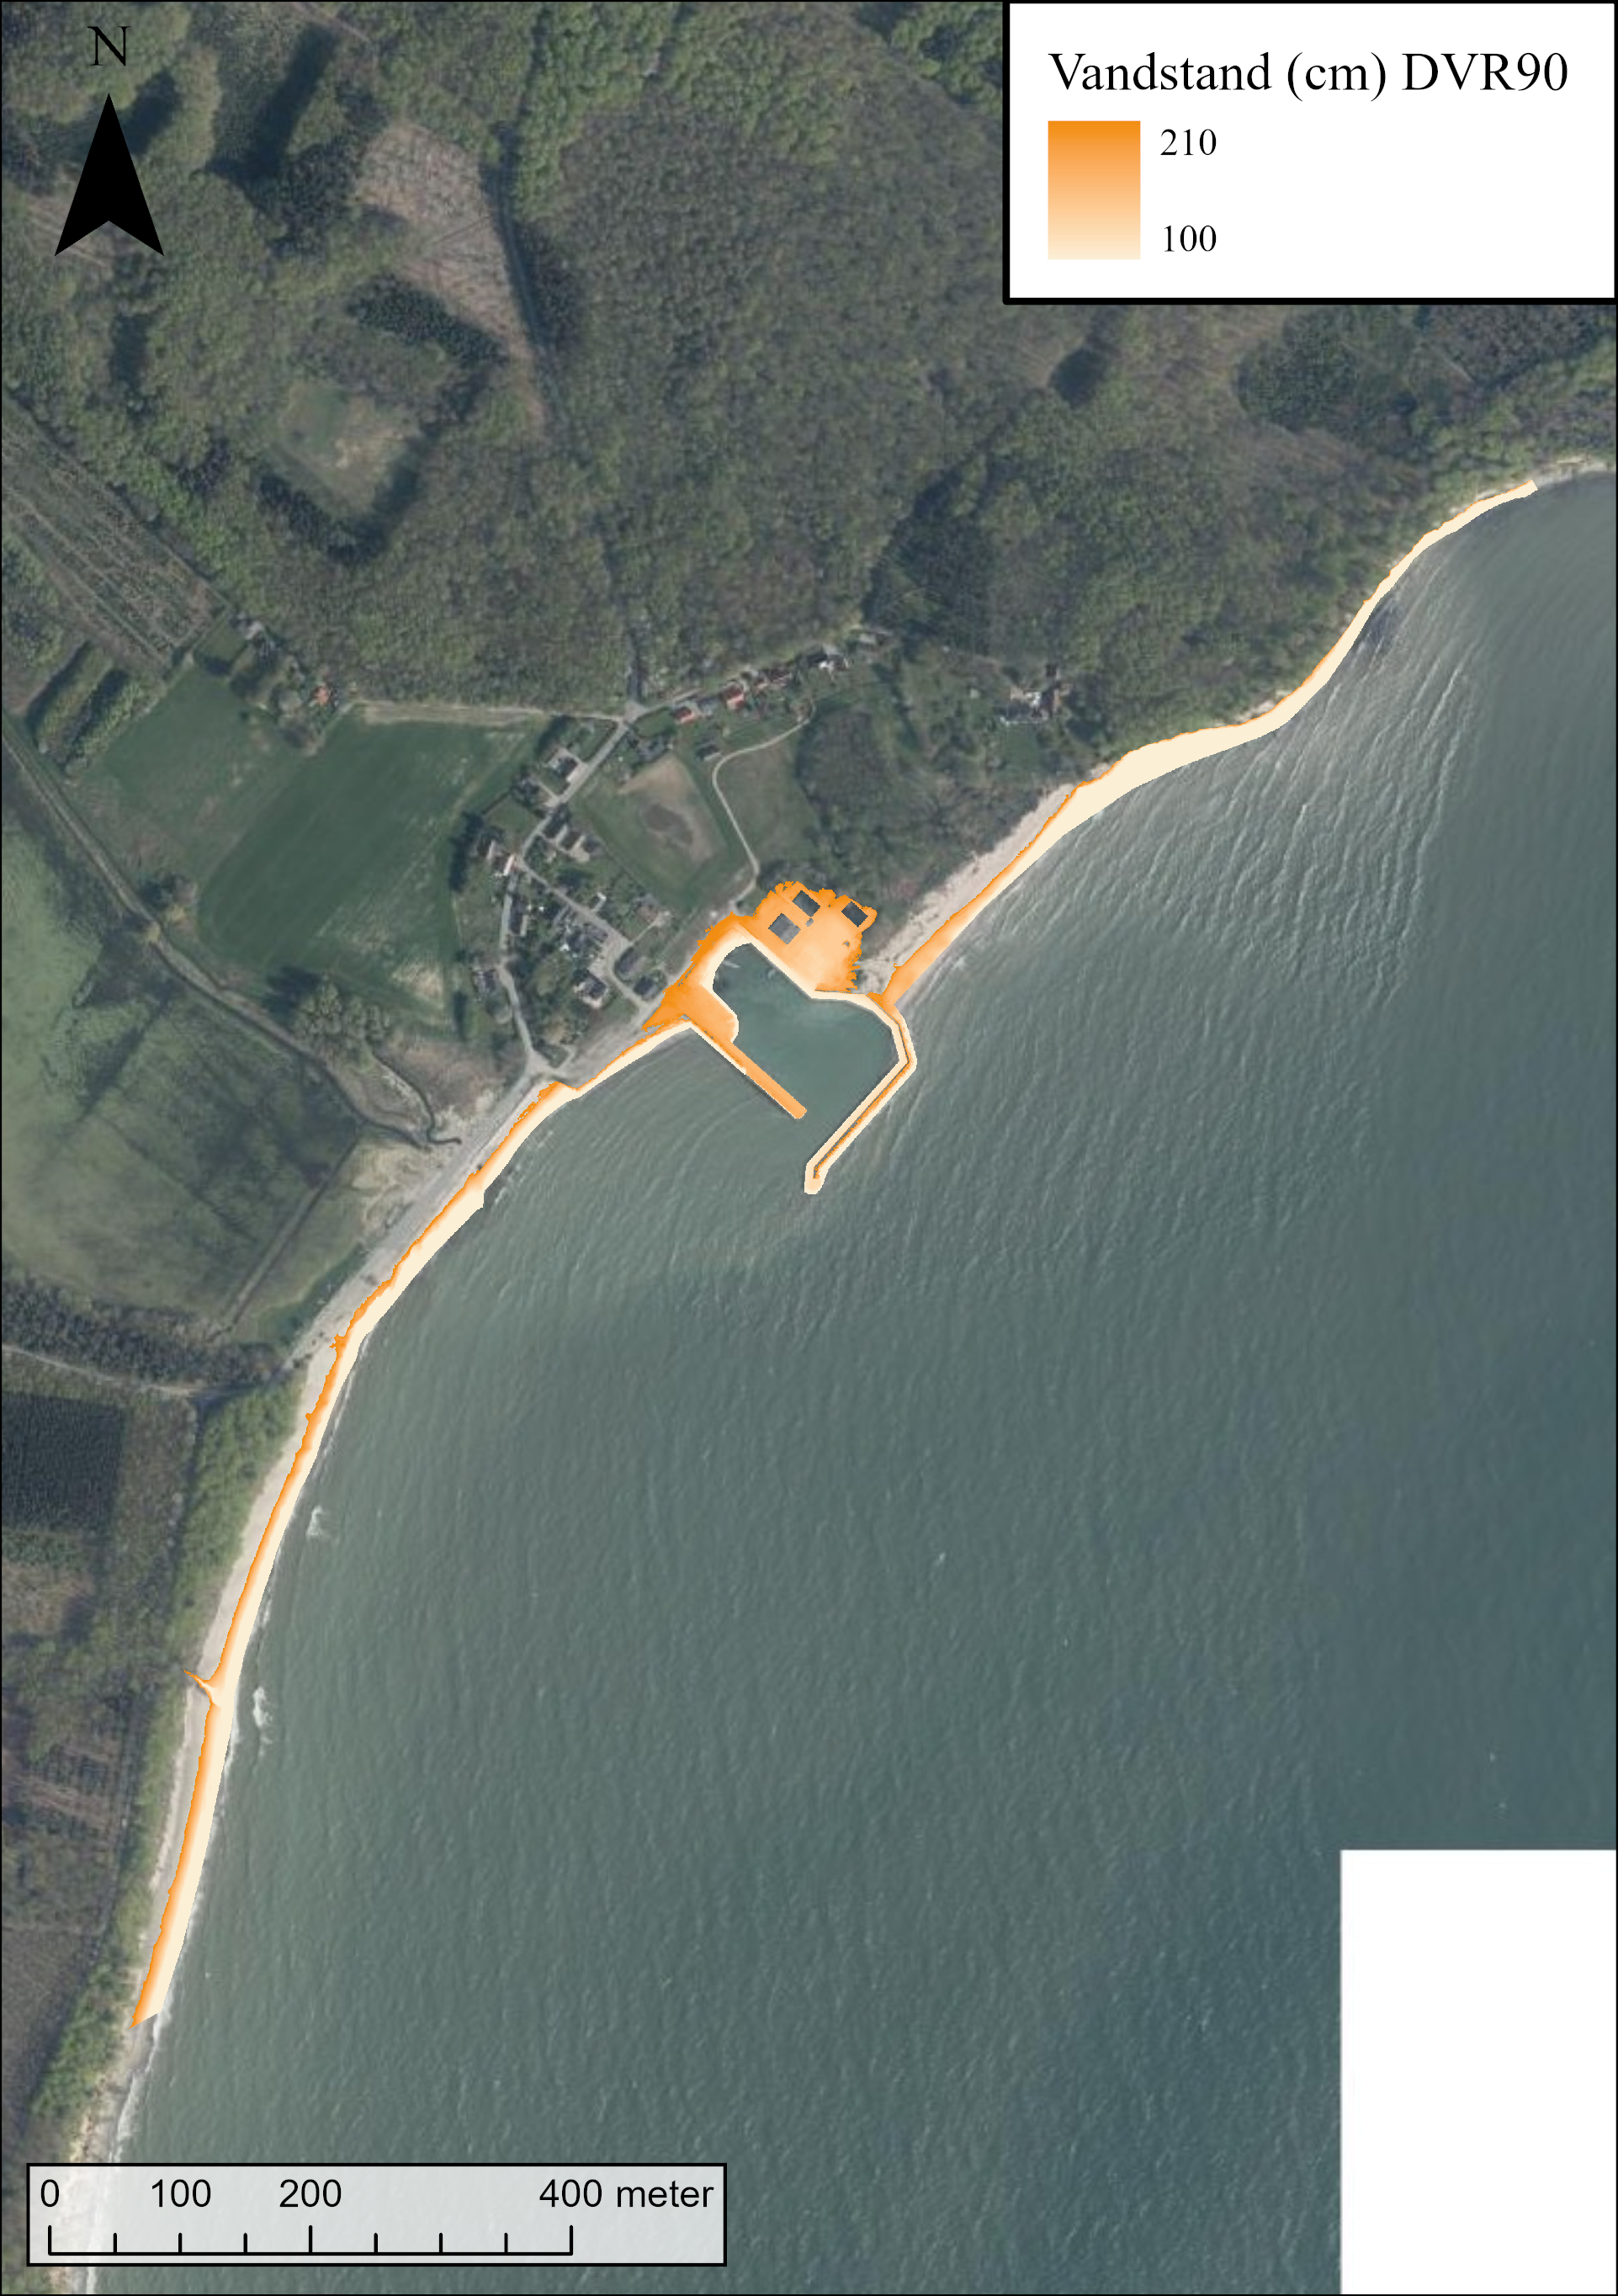
\includegraphics[width=0.8\linewidth]{images/Resultater/2023Model/2023 model_hesnaes.jpg}
        \caption{Simuleret oversvømmelseskort over Hesnæs}
        \label{Subfig: Model Hesnæs}
    \end{subfigure}
    \caption{Målt og simuleret oversvømmelseskort af oktober 2023 stormfloden for Hesnæs i centimeter over DVR90}
    \label{Figur: Målt & simuleret Hesnæs}
\end{figure}

I Hesnæs blev der påvirket seks forskellige arealanvendelser. De mest påvirkede arealer i Hesnæs har primært været kysten, der falder ind under naturområder. Dette har været gældende for begge resultater. Den målte hændelse med 66,2\% og den simulerede hændelse med 65,8\% oversvømmet naturområder. Bebyggede områder blev oversvømmet med 11,9 og 12,1\% og infrastruktur med 10,7 og 11,5\% respektivt for den målte hændelse og det simuleret resultat.  

\begin{figure}[H]
    \centering
    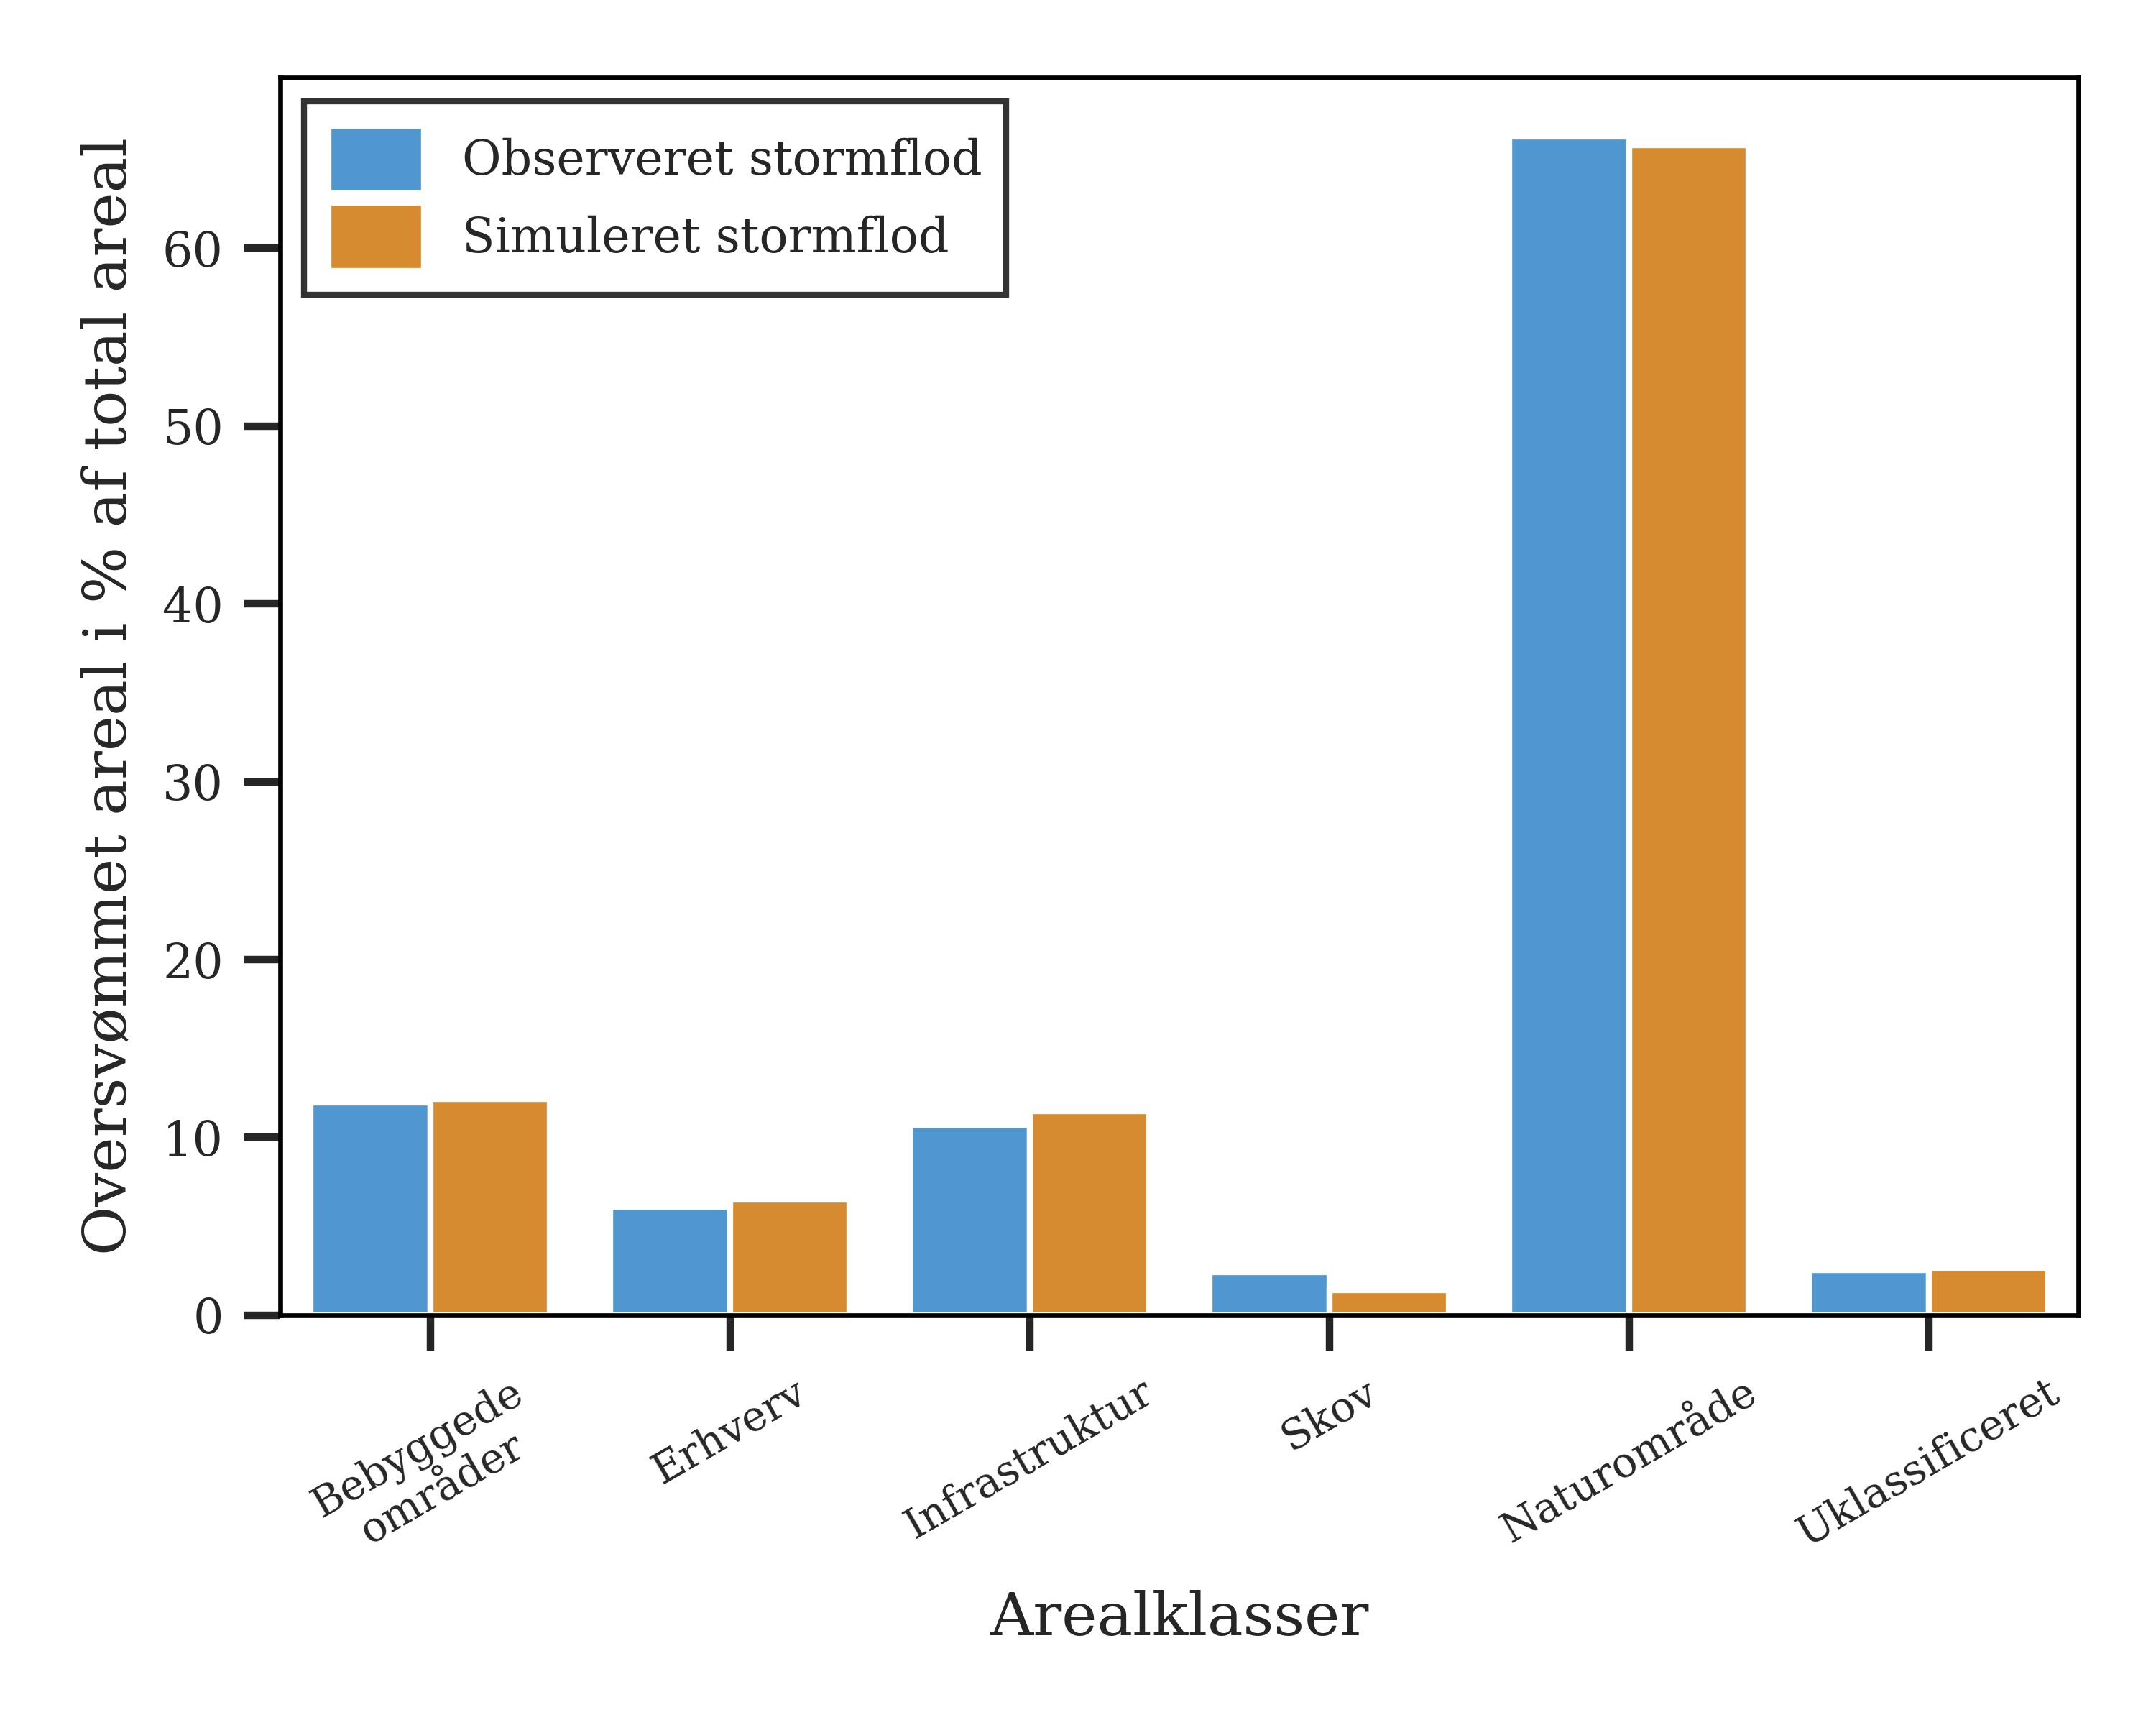
\includegraphics[width=0.8\linewidth]{images/Resultater/areal_anvendelses_grafer/hesnaes_arealanvendelse.jpg}
    \caption{Påvirkede arealanvendelsesklasser som procent af totalt oversvømmet areal i Hesnæs for den målte og simuleret oktober 2023 stormflods hændelse}
    \label{Figur: Påvirket arealanvendelse Hesnæs}
\end{figure}

Figur \ref{Figur: Målt & simuleret Præstø} viser den målte 2023 stormflods hændelse og den simuleret hændelse i Præstø. Begge kort viser at kysten og havnen af Præstø bliver oversvømmet og lidt af den nordlige bydel. Den største forskel mellem de to kort er at under den målte hændelse er en stor del af Tubæk Ådal oversvømmet, da sluseporten fra Tubæk Ådal ud til Præstø Fjord kollapsede under vandpresset. Den målte hændelse på 534967 m\textsuperscript{2} er derfor 25,53\% større i udbredelse end det simuleret resultat på 398365 m\textsuperscript{2}, svarende til 136602 m\textsuperscript{2}. 

\begin{figure}[H]
    \begin{subfigure}[t]{0.5\textwidth}
        \centering
        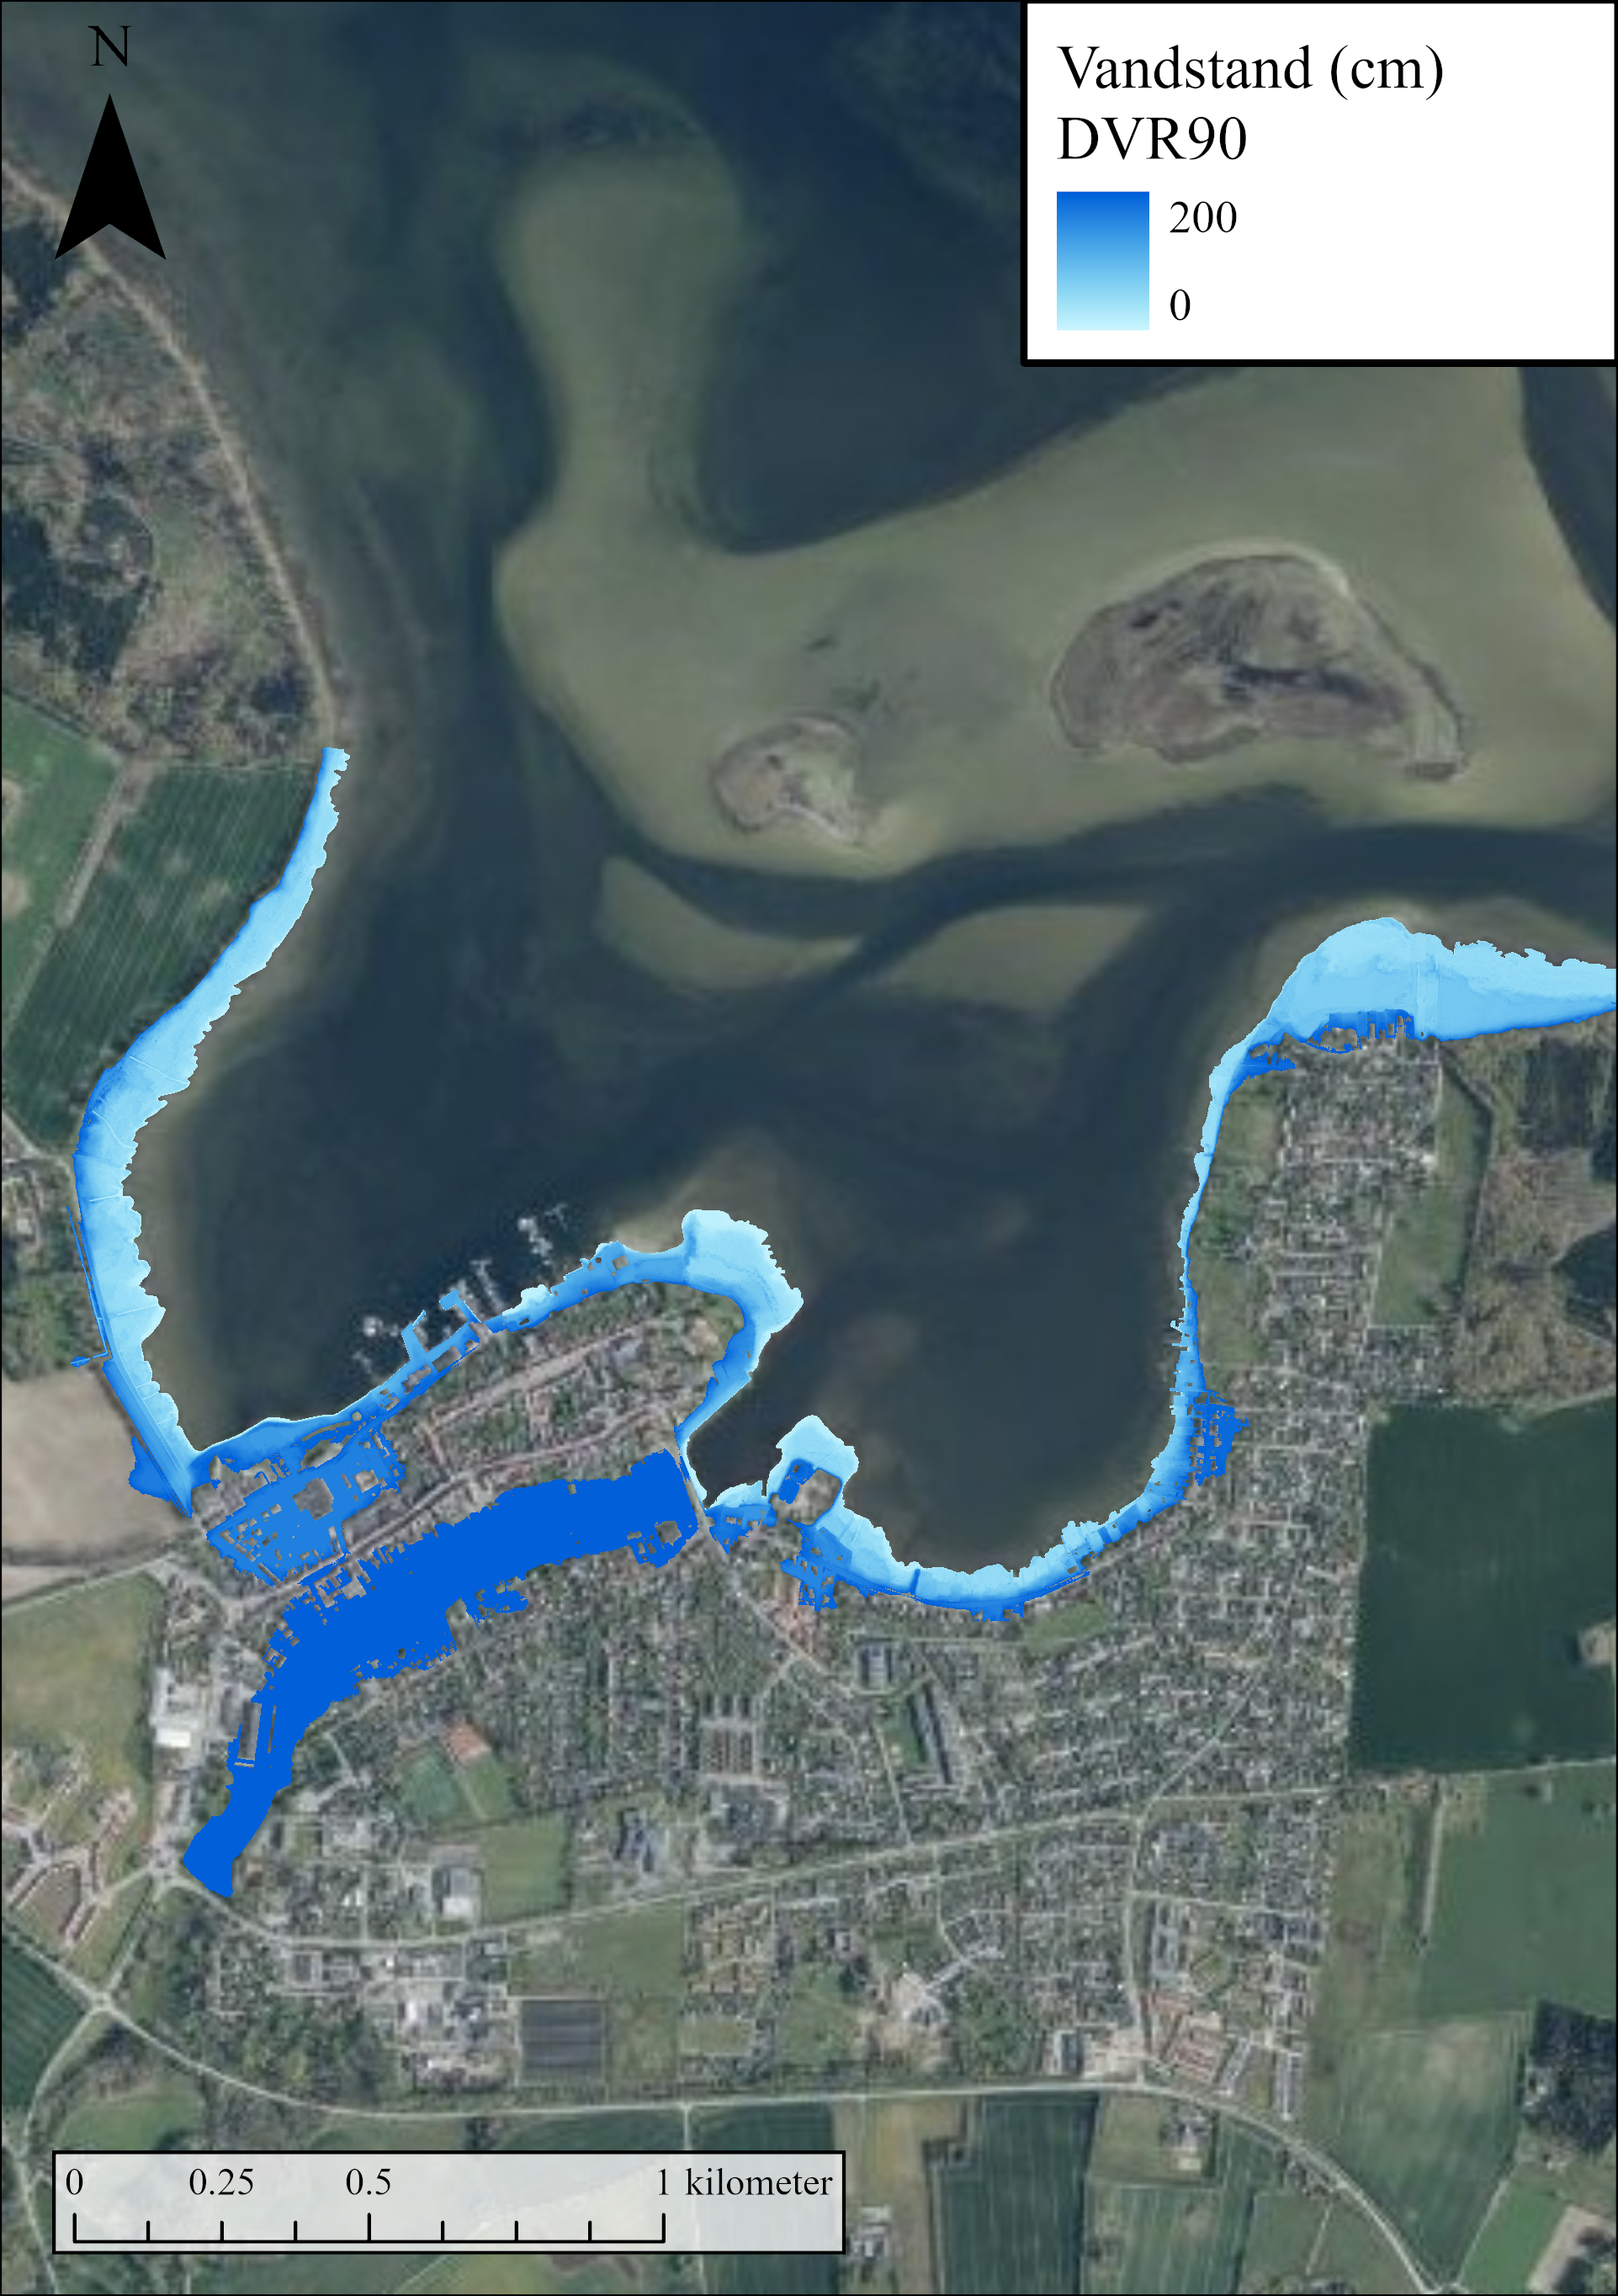
\includegraphics[width=0.8\linewidth]{images/Resultater/2023Malt/2023 resultat_praestoe.jpg}
        \caption{Målte oversvømmelseskort over Præstø}
        \label{Subfig: Målt Præstø}
    \end{subfigure}
    \begin{subfigure}[t]{0.5\textwidth}
        \centering
        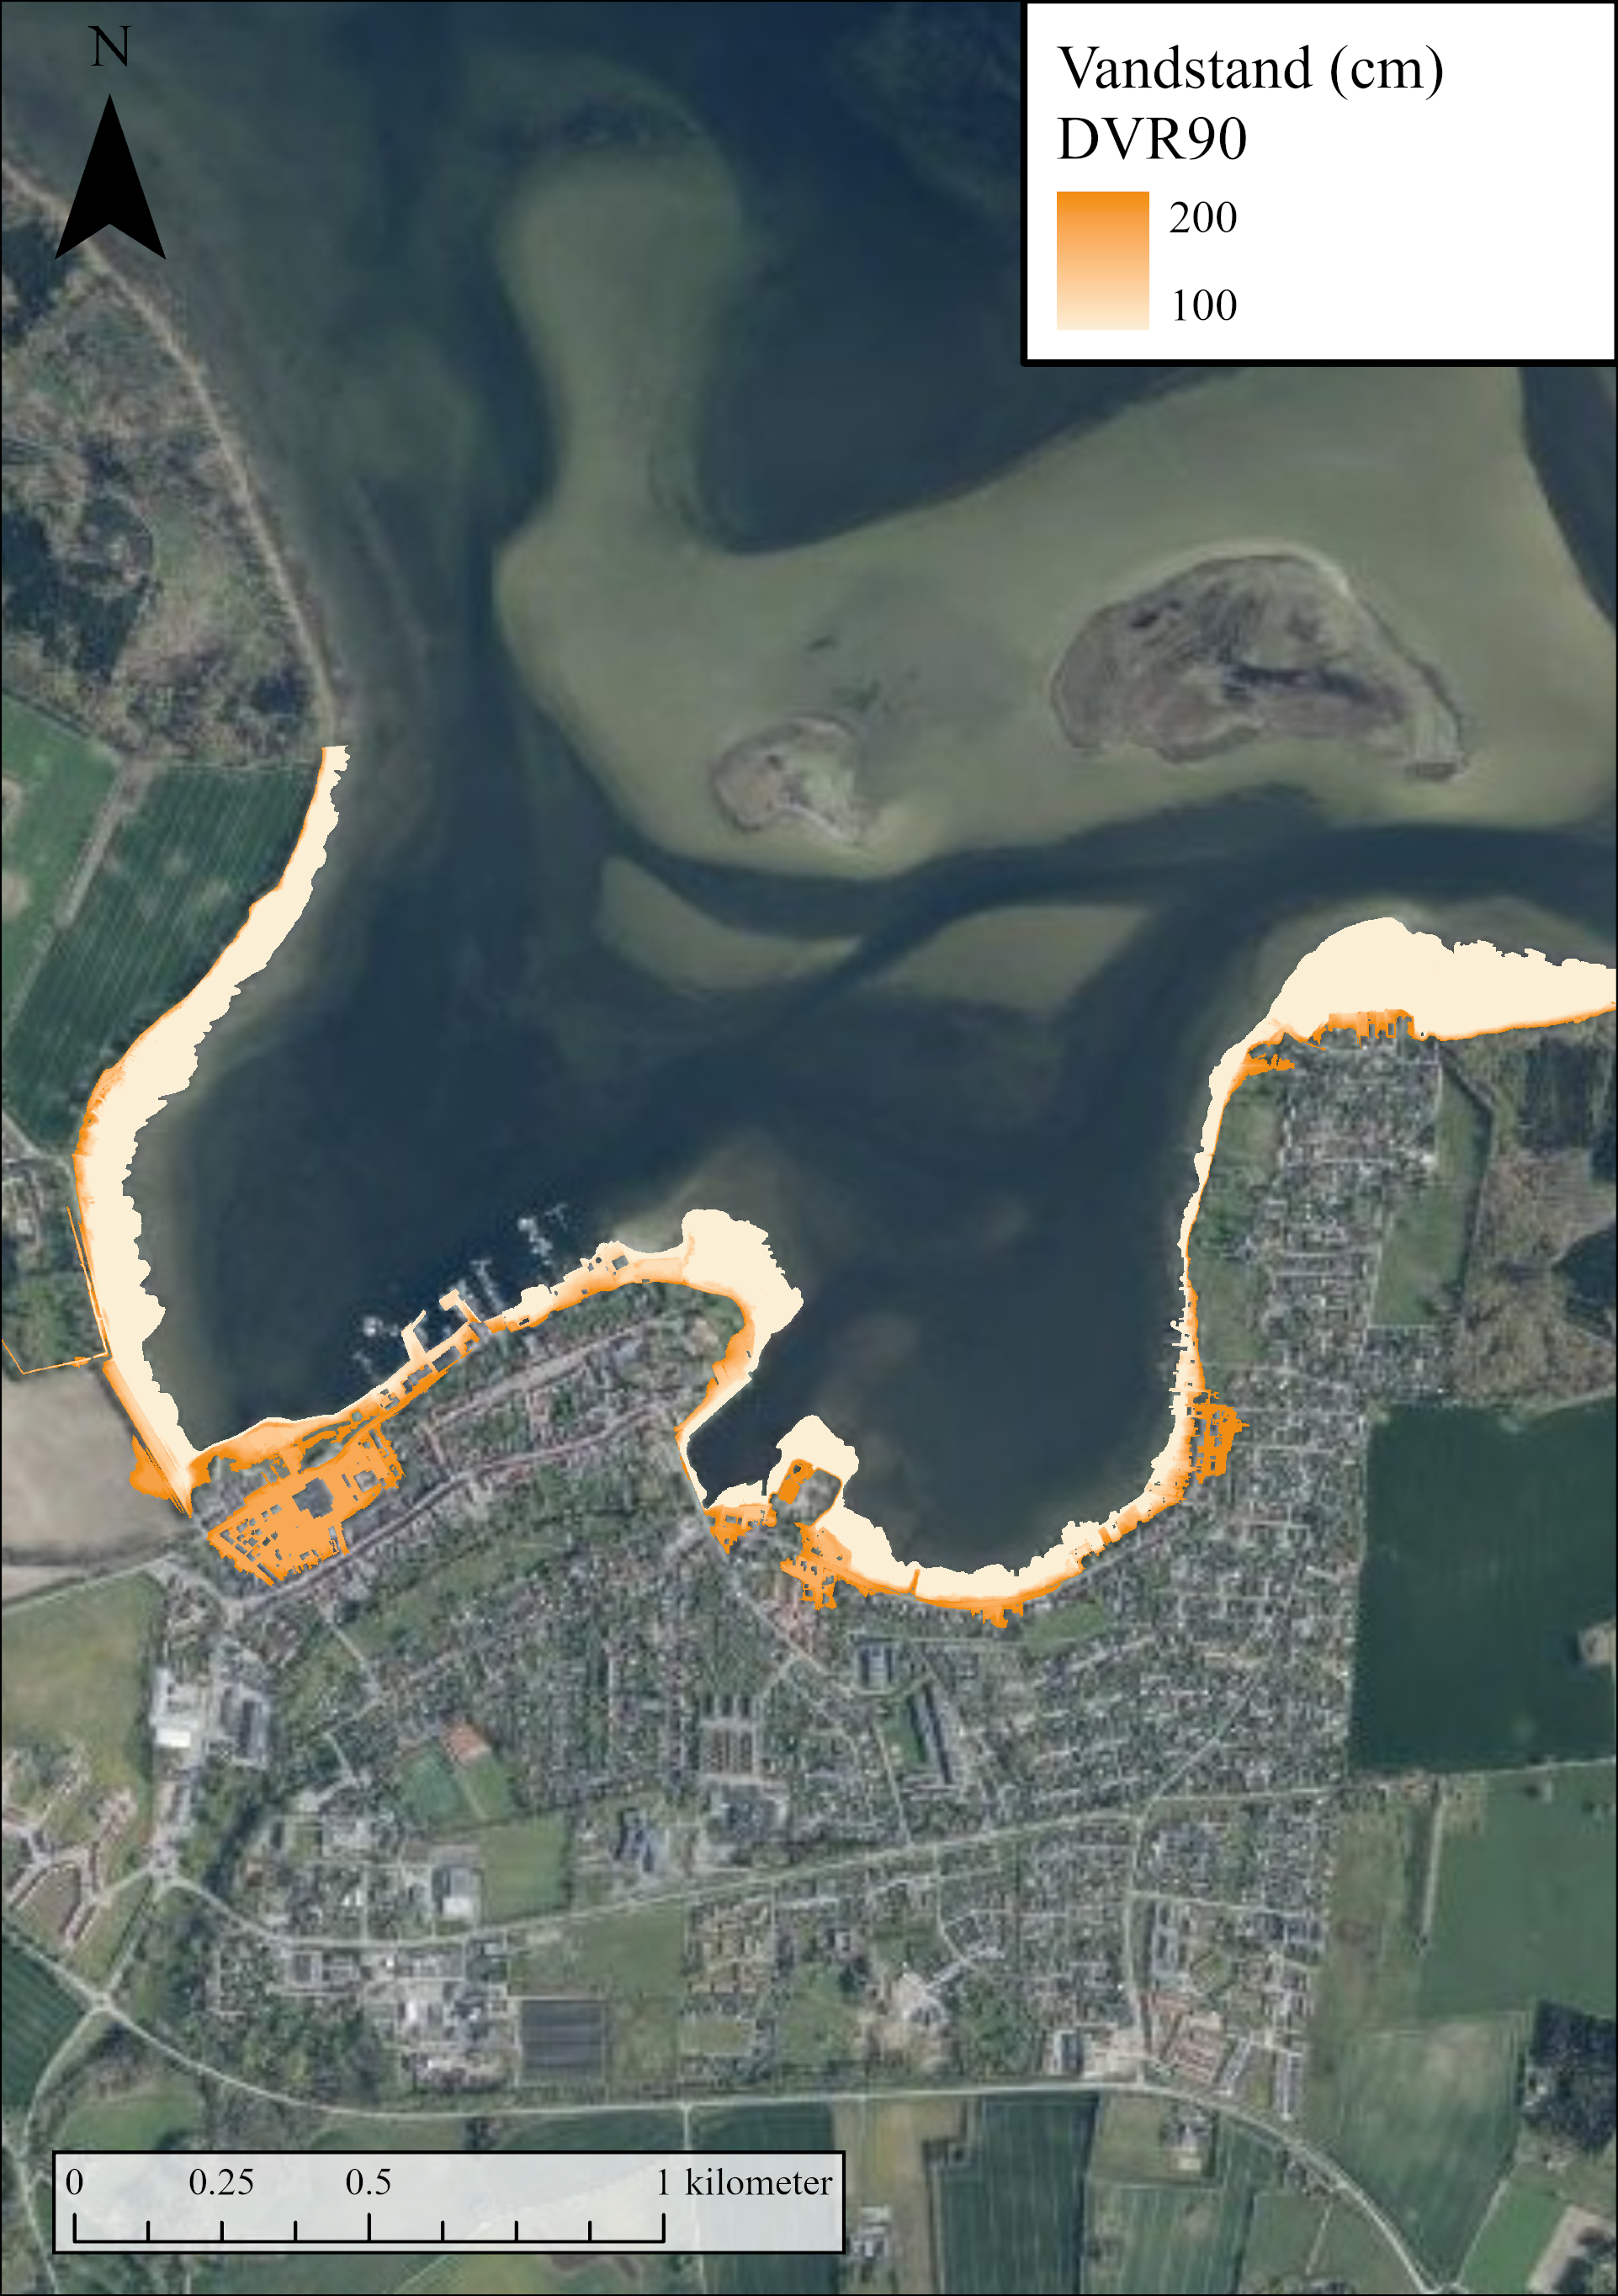
\includegraphics[width=0.8\linewidth]{images/Resultater/2023Model/2023 model_praestoe.jpg}
        \caption{Simuleret oversvømmelseskort over Præstø}
        \label{Subfig: Model Præstø}
    \end{subfigure}
    \caption{Målt og simuleret oversvømmelseskort af oktober 2023 stormfloden for Præstø i centimeter over DVR90}
    \label{Figur: Målt & simuleret Præstø}
\end{figure}

I Præstø blev otte forskellige arealanvendelser påvirket af 2023 stormfloden. For både den målte og den simuleret hændelse var naturområder det mest påvirket areal med 46,9 og 60,4\% henholdsvis (\ref{Figur: Påvirket arealanvendelse Præstø}). Den målte hændelse havde et større rekreativt areal oversvømmet end den simuleret hændelse med en forskel på 40633,4 m\textsuperscript{2}, da arealerne langs Tubæk Ådal er klassificeret som rekreative områder. Grundet oversvømmelsen af Tubæk Ådal har der været flere bebyggede områder, såsom huse og lejligheder der blev oversvømmet ved den målte hændelse, som ikke blev oversvømmet i resultatet fra Inundation Modellen. 

\begin{figure}[H]
    \centering
    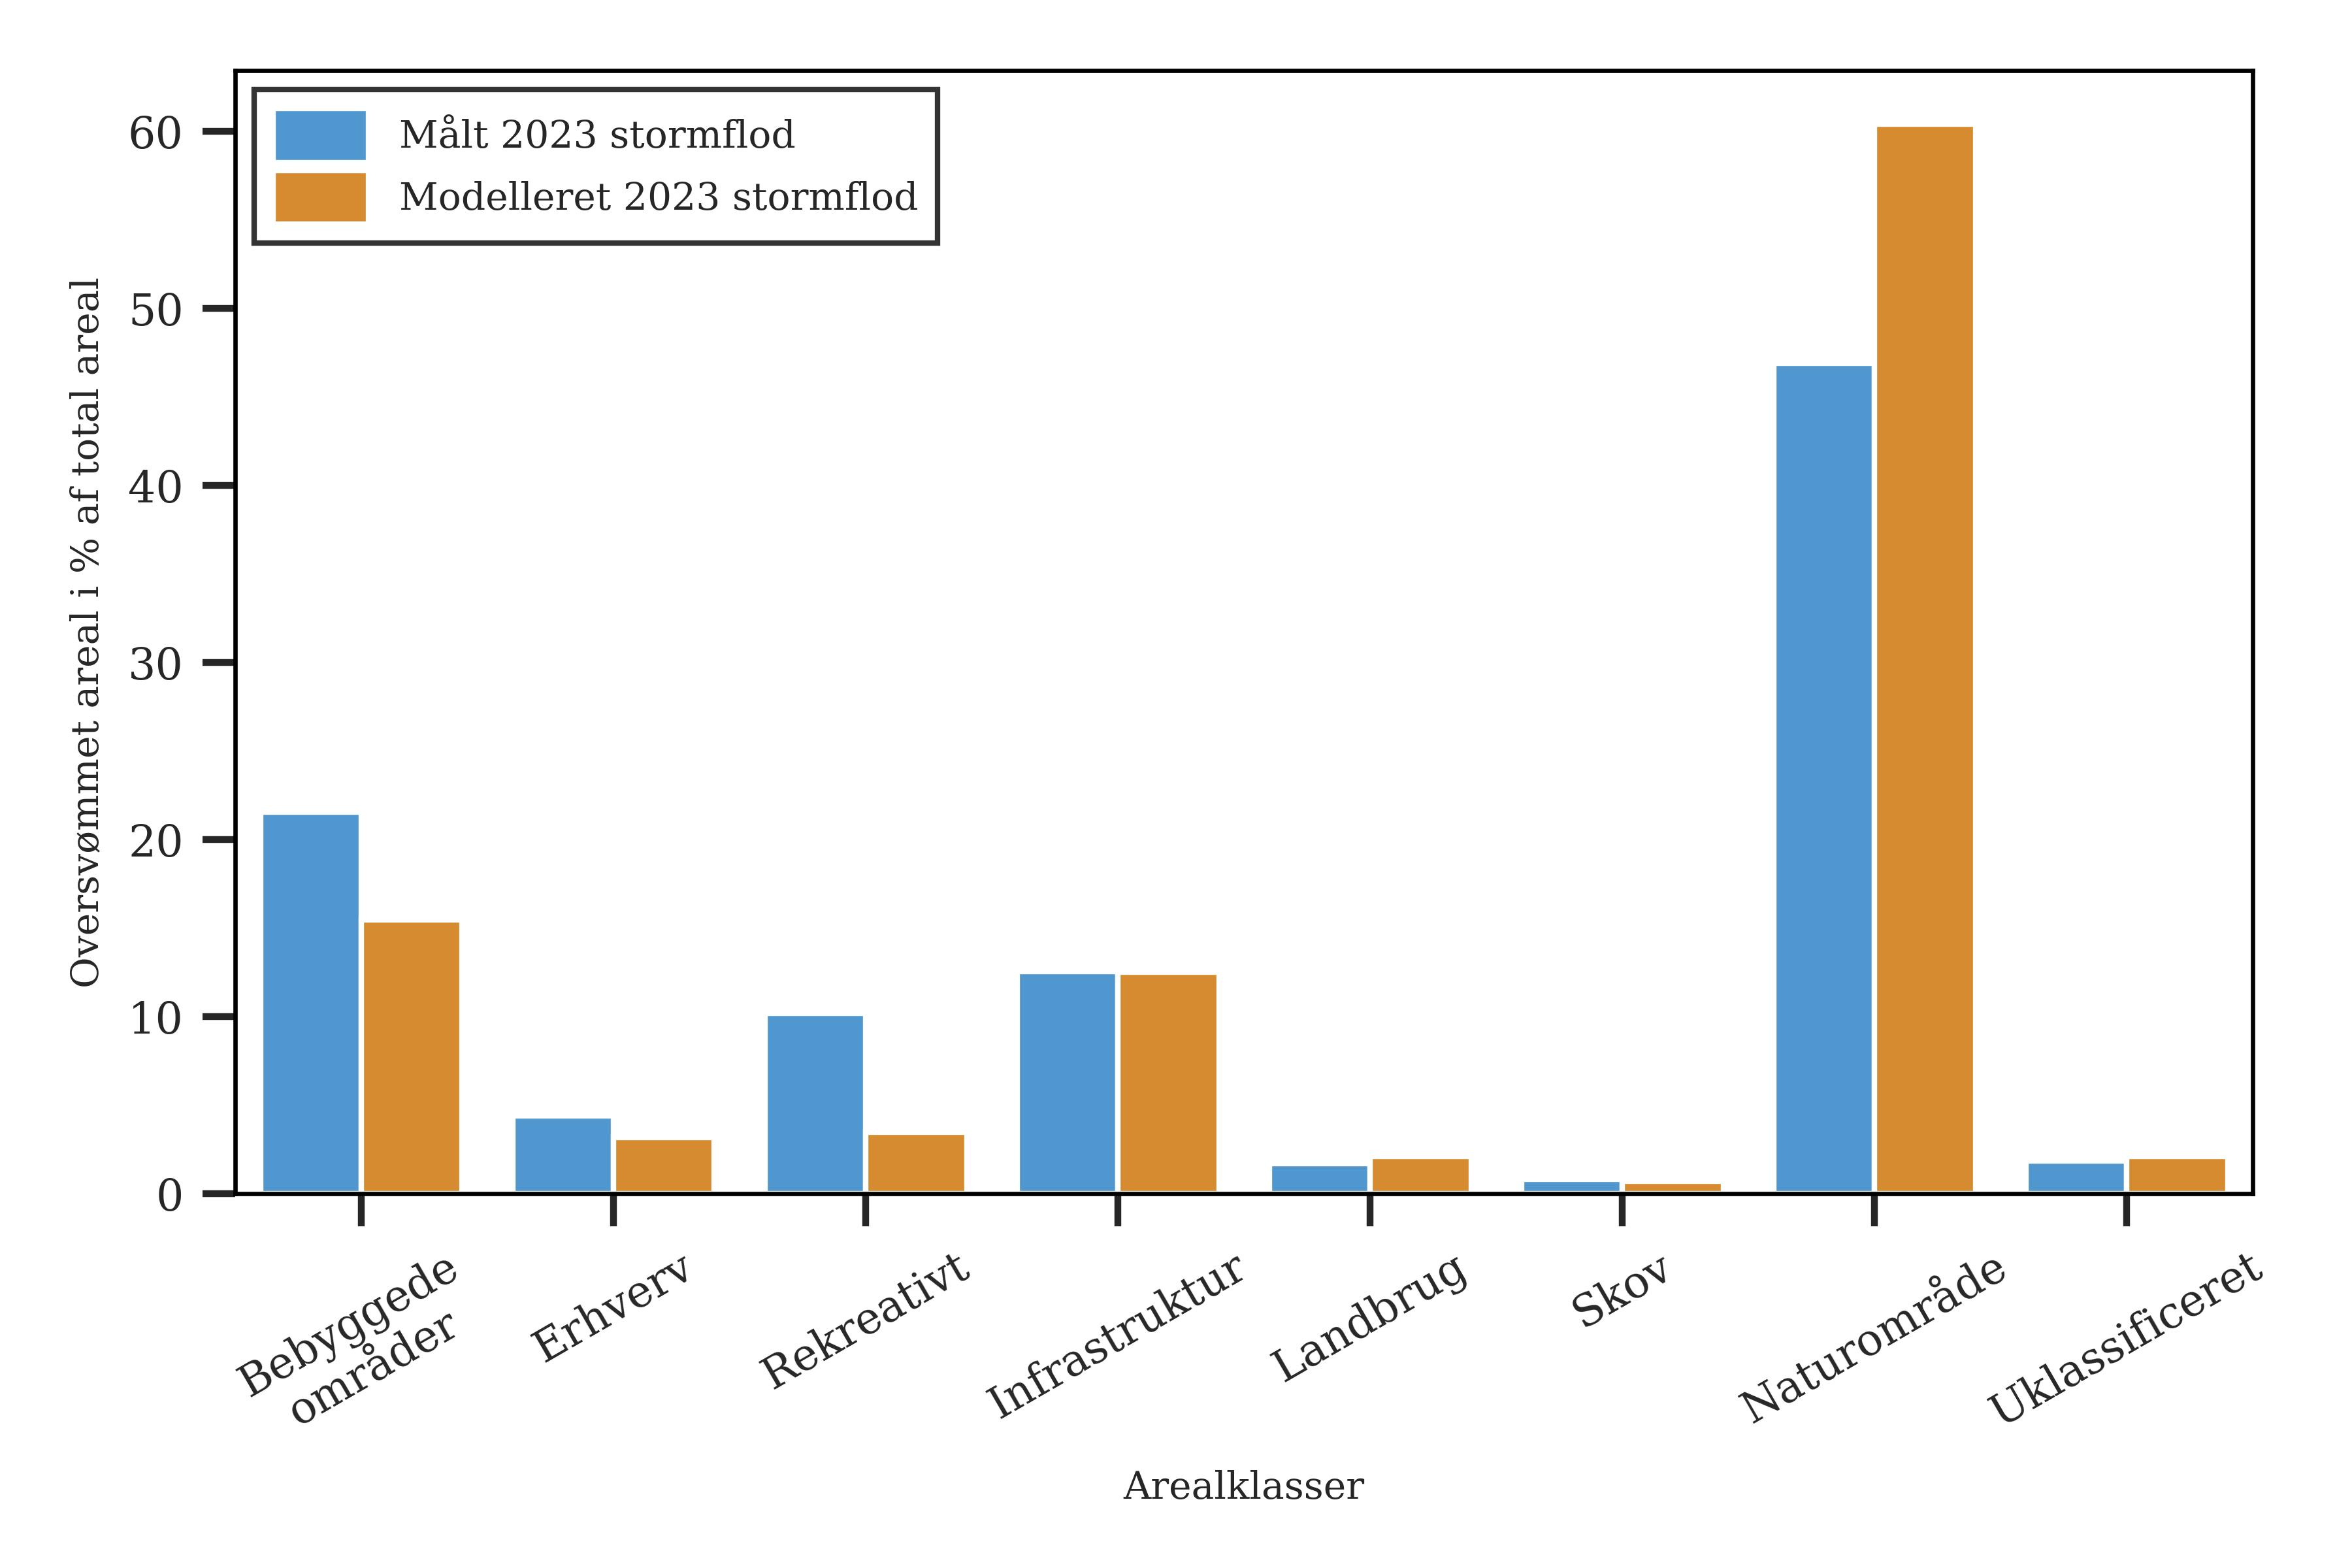
\includegraphics[width=0.8\linewidth]{images/Resultater/areal_anvendelses_grafer/praestoe_arealanvendelse.jpg}
    \caption{Påvirkede arealanvendelsesklasser som procent af totalt oversvømmet areal i Præstø for den målte og simuleret oktober 2023 stormflods hændelse}
    \label{Figur: Påvirket arealanvendelse Præstø}
\end{figure}

I Gedser og Hesnæs simulerede Inundation Modellen stormflods hændelsen fra oktober 2023 fornuftigt med relative nøjagtige gengivelser af vandets udbredelse, mens Aabenraa og Præstø blev simuleret mindre præcist grundet eksogene faktorer såsom beredskabstiltag og kollaps af stormflodssikringer. 

\subsection{Fremskrevet og statistiske stormflods hændelser}

I denne sektion vil der blive præsenteret resultaterne  af en statistisk 100-års hændelse og en fremskrivning af oktober 2023 stormfloden ved SSP4,5 og 8,5. \\

I figur \ref{Figur: Klima Aabenraa} ses et oversvømmelseskort over Aabenraa for en statistisk 100-års hændelse og en fremskrivning af 2023 stormfloden ved et SSP4,5 og SSP8,5 scenarie. Det største areal oversvømmet sker ved en vandstand på 234 cm over DVR90. En større del af den sydlige bydel bliver oversvømmet ved en statistisk 100-års hændelse i et SSP4,5 scenarie. Oversvømmet areal ved fremskrivningen af oktober 2023 stormfloden i et SSP8,5 scenarie er 13\% større end en statistisk 100-års hændelse i SSP4,5. Det svarer til 196489,45 m\textsuperscript{2}. I forhold til den målte stormflodshændelse i 2023, oversvømmer en fremskrevet stormflod 136 og 147\% areal ved henholdsvis SSP4,5 og SSP8,5.
\begin{figure}[H]
    \centering
    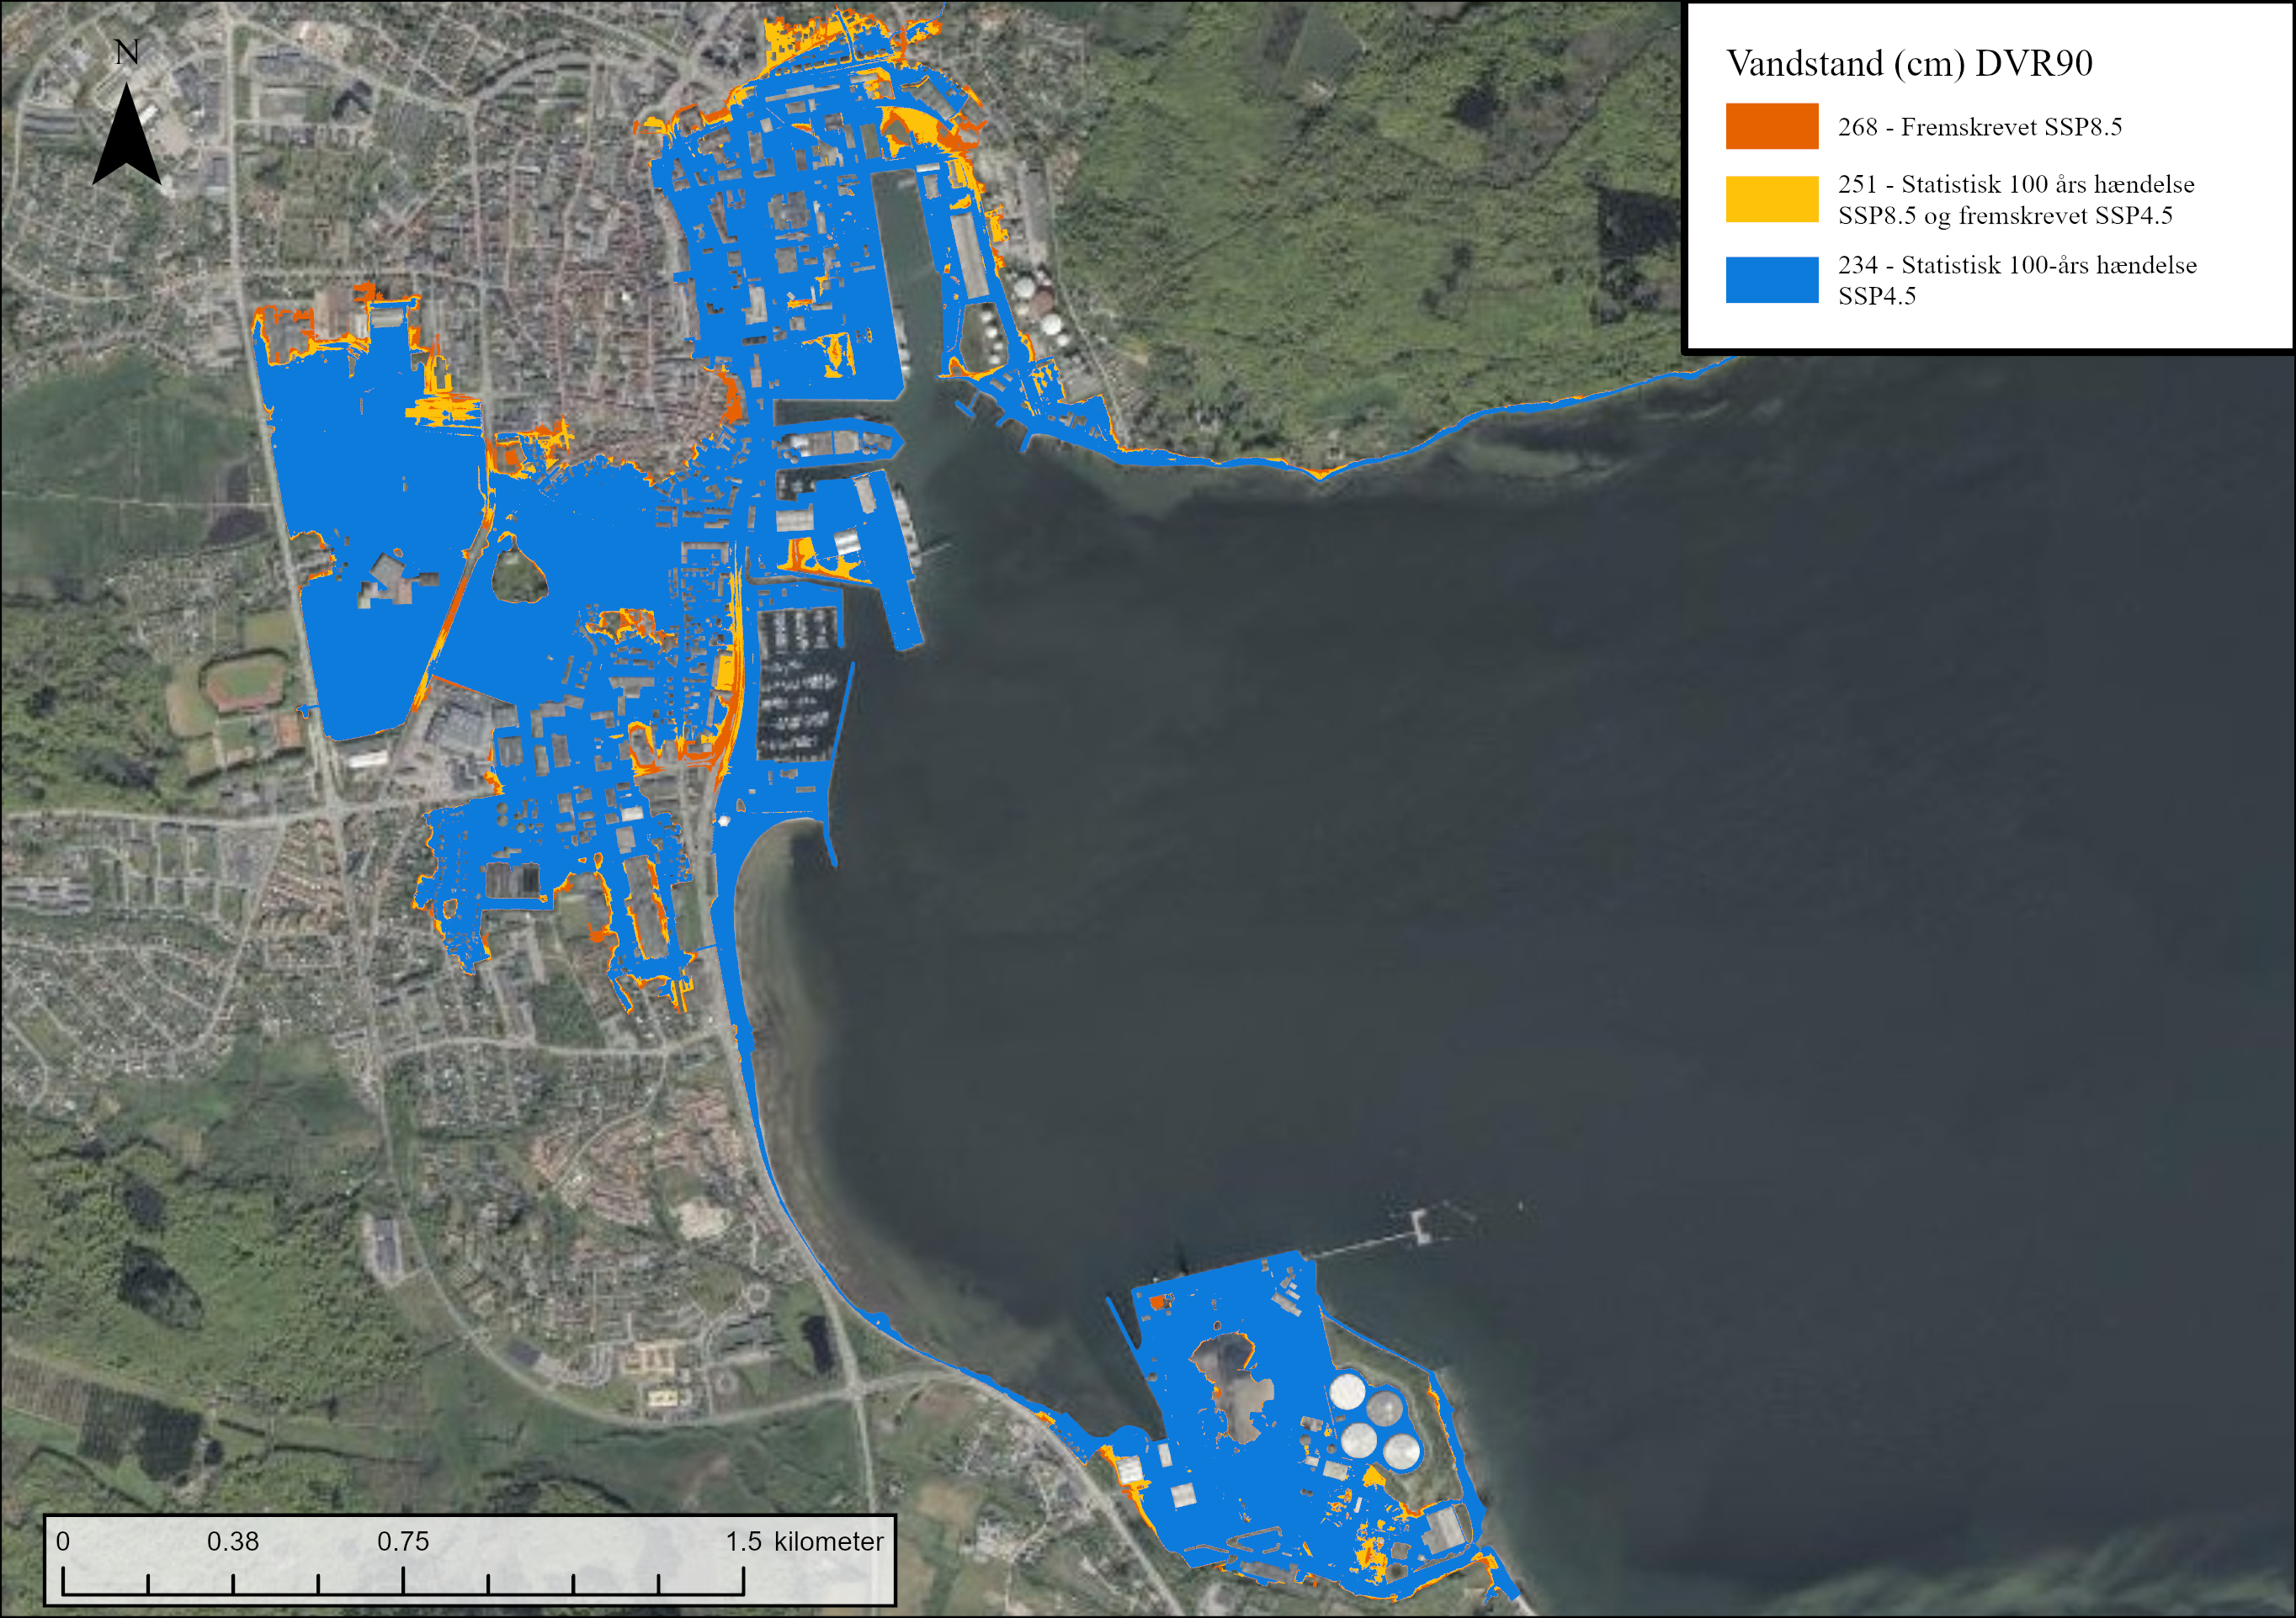
\includegraphics[width=0.8\linewidth]{images/Resultater/fremskrevet_hændelser/klima resultat_aabenraa.jpg}
    \caption{Kort over oversvømmet areal i Aabenraa af en stormflod ved en statistisk 100-års hændelse og en fremskrivning af oktober 2023 stormfloden til slutningen af århundredet ved SSP4,5 og SSP8,5 i centimeter over DVR90}
    \label{Figur: Klima Aabenraa}
\end{figure}

I figur \ref{Figur: Klima Gedser Havn} er der vist et oversvømmelseskort over Gedser Havn for en statistisk 100-års hændelse og fremskrivningen af oktober 2023 stormfloden ved et SSP4,5 og 8,5 scenarie. Den største del af oversvømmelsen sker ved en fremskrevet 2023 stormflod ved SSP4,5 med en vandstand på 220 cm DVR90. Meget af landsbyen Gedser Havn bliver oversvømmet og en stor del af det bagvedliggende landbrugsområder. Ved en statistisk 100-års hændelse i et SSP8,5 scenarie er det oversvømmet areal steget til 2196903,3 m\textsuperscript{2}, en stigning på 537\% i forhold til den stormflod der ramte i oktober 2023. 

\begin{figure}[H]
    \centering
    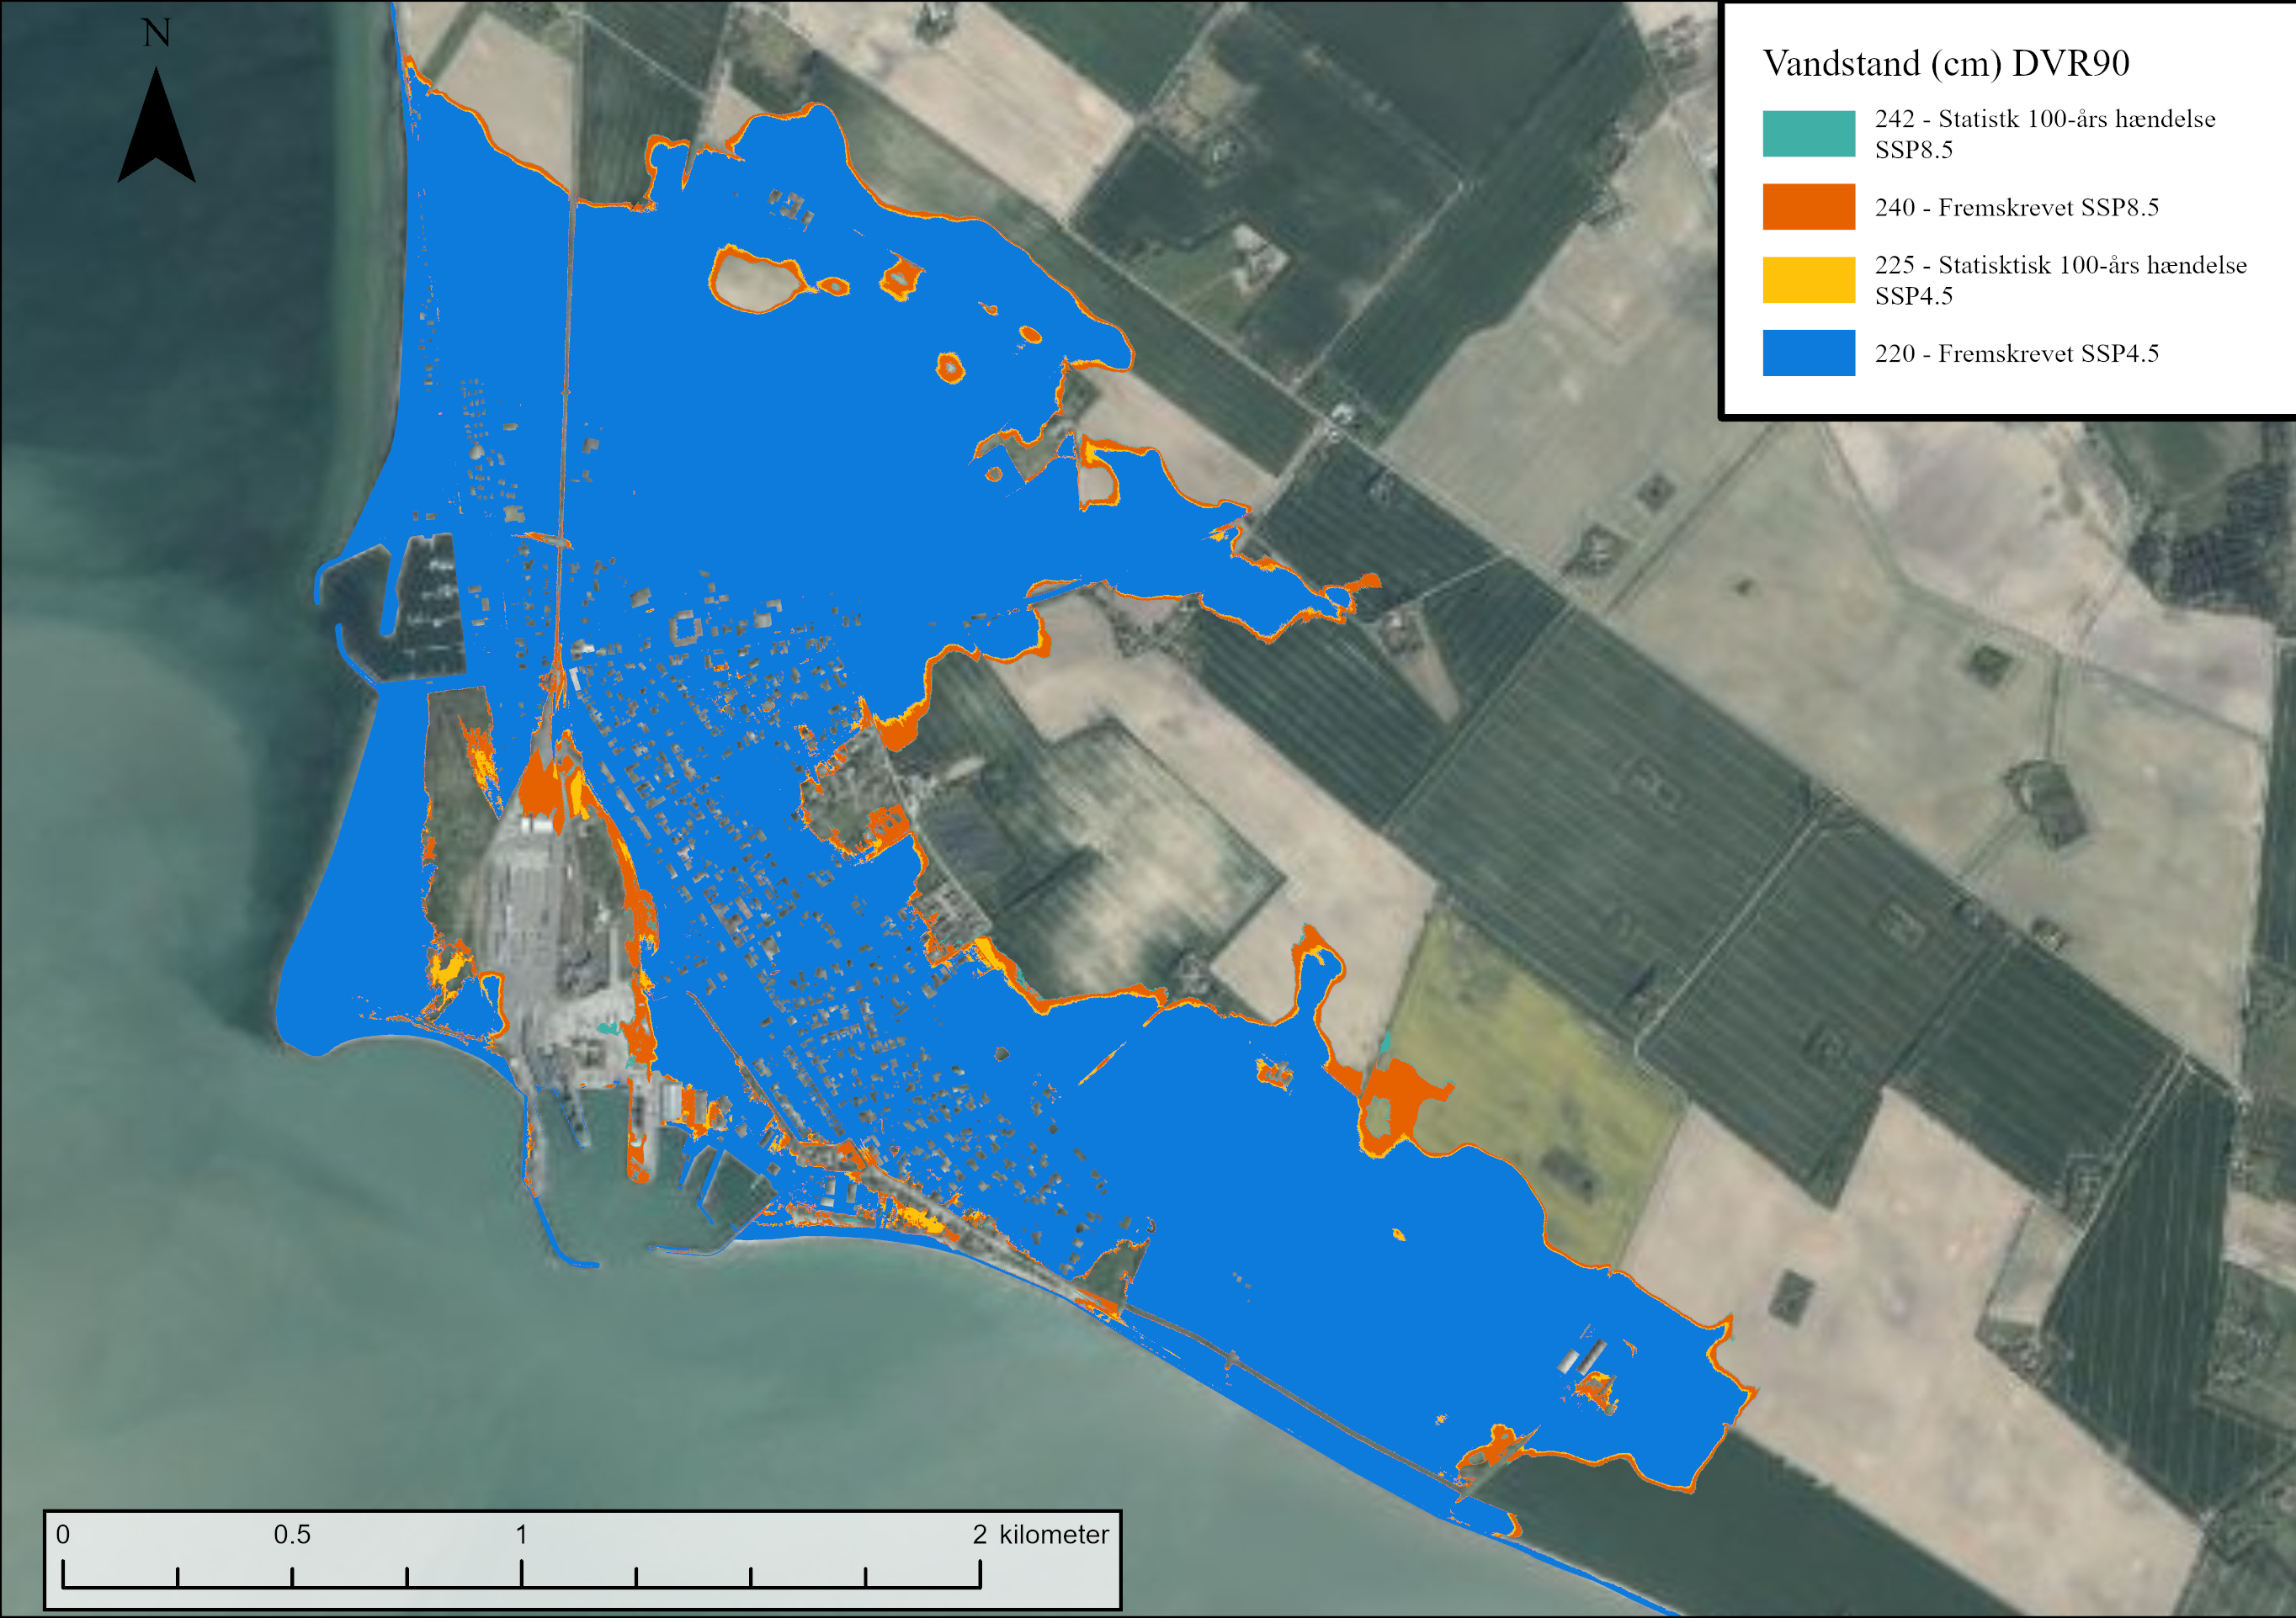
\includegraphics[width=0.8\linewidth]{images/Resultater/fremskrevet_hændelser/klima resultat gedser.jpg}
    \caption{Kort over oversvømmet areal i Gedser Havn af en stormflod ved en statistisk 100-års hændelse og en fremskrivning af oktober 2023 stormfloden til slutningen af århundredet ved SSP4,5 og SSP8,5 i centimeter over DVR90}
    \label{Figur: Klima Gedser Havn}
\end{figure}

I Hesnæs bliver et stort lavliggende græsareal oversvømmet ved en statistisk 100-års hændelse i et SSP8,5 scenarie. Ved en 100-års hændelse i SSP4,5 oversvømmes det meste af kysten og havnen. Selve Hesnæs by er udenfor oversvømmelsesrisiko selv ved det højeste vandstandsniveau på 259 cm DVR90 (figur \ref{Figur: Klima Hesnæs}). Ved en oversvømmelse i et SSP8,5 scenarie vil det oversvømmede areal stige fra 48292,7 m\textsuperscript{2} til 1147615,2 m\textsuperscript{2}. Dette er en stigning på 2305\%. \\
Ved en fremskrevet 2023 stormflod vil der oversvømmes et areal der er 3219\% større end det der blev målt under stormfloden den 20. oktober 2023. 

\begin{figure}[H]
    \centering
    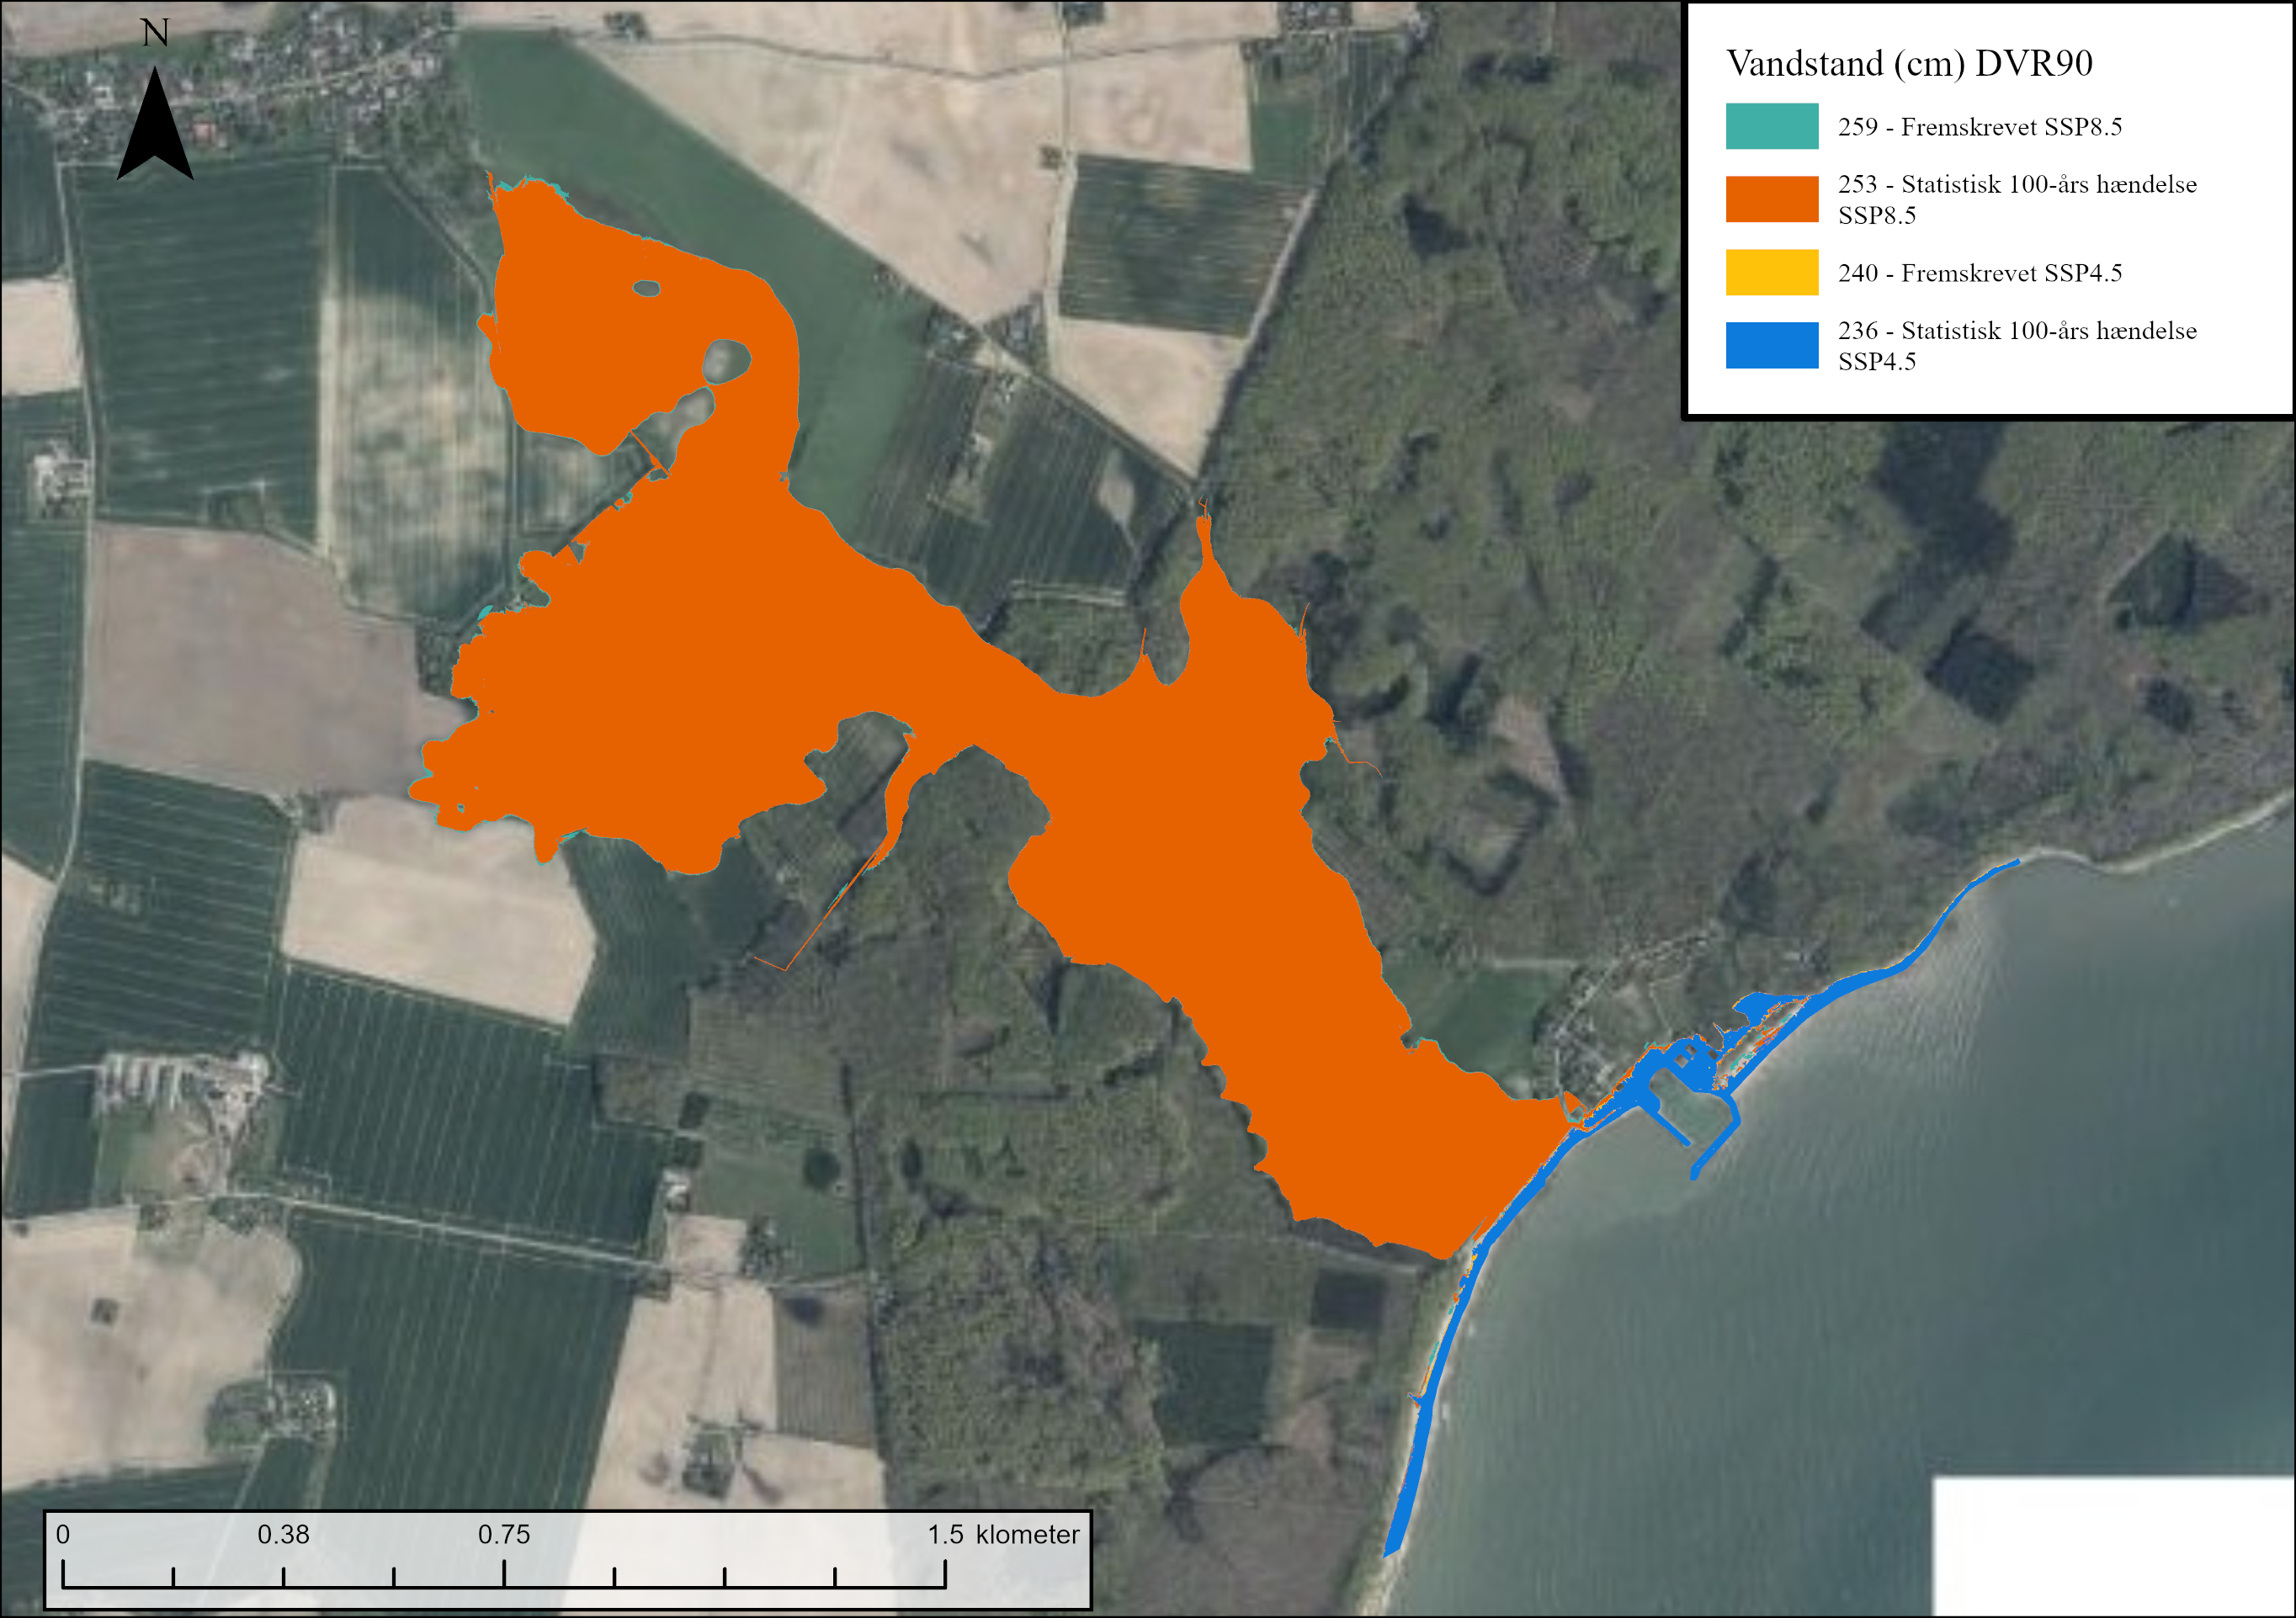
\includegraphics[width=0.8\linewidth]{images/Resultater/fremskrevet_hændelser/klima resultat hesnaes.jpg}
    \caption{Kort over oversvømmet areal i Hesnæs af en stormflod ved en statistisk 100-års hændelse og en fremskrivning af oktober 2023 stormfloden til slutningen af århundredet ved SSP4,5 og SSP8,5 i centimeter over DVR90}
    \label{Figur: Klima Hesnæs}
\end{figure}

I figur \ref{Figur: Klima Præstø} er der visualiseret vandets udbredelse ved en statistisk 100-års hændelse og en fremskrevet 2023 stormflod i et SSP4,5 og 8,5 scenarie. Ved en 100-års SSP4,5 hændelse bliver store dele af Præstø by oversvømmet, både nord og syd for Tubæk Ådal. Meget af Tubæk Ådal vil også blive lagt under vand og åen vil gå over sine bredder i den sydlige del af byen. Et areal der er 68\% større end stormfloden der oversvømmede byen i 2023 vil blive oversvømmet hvis den samme stormflod rammer Præstø i slutningen af dette århundrede i et SSP8,5 scenarie. Dette vil være en stigning på 56550 m\textsuperscript{2} i forhold til en 100-års hændelse i SSP4,5.

\begin{figure}[H]
    \centering
    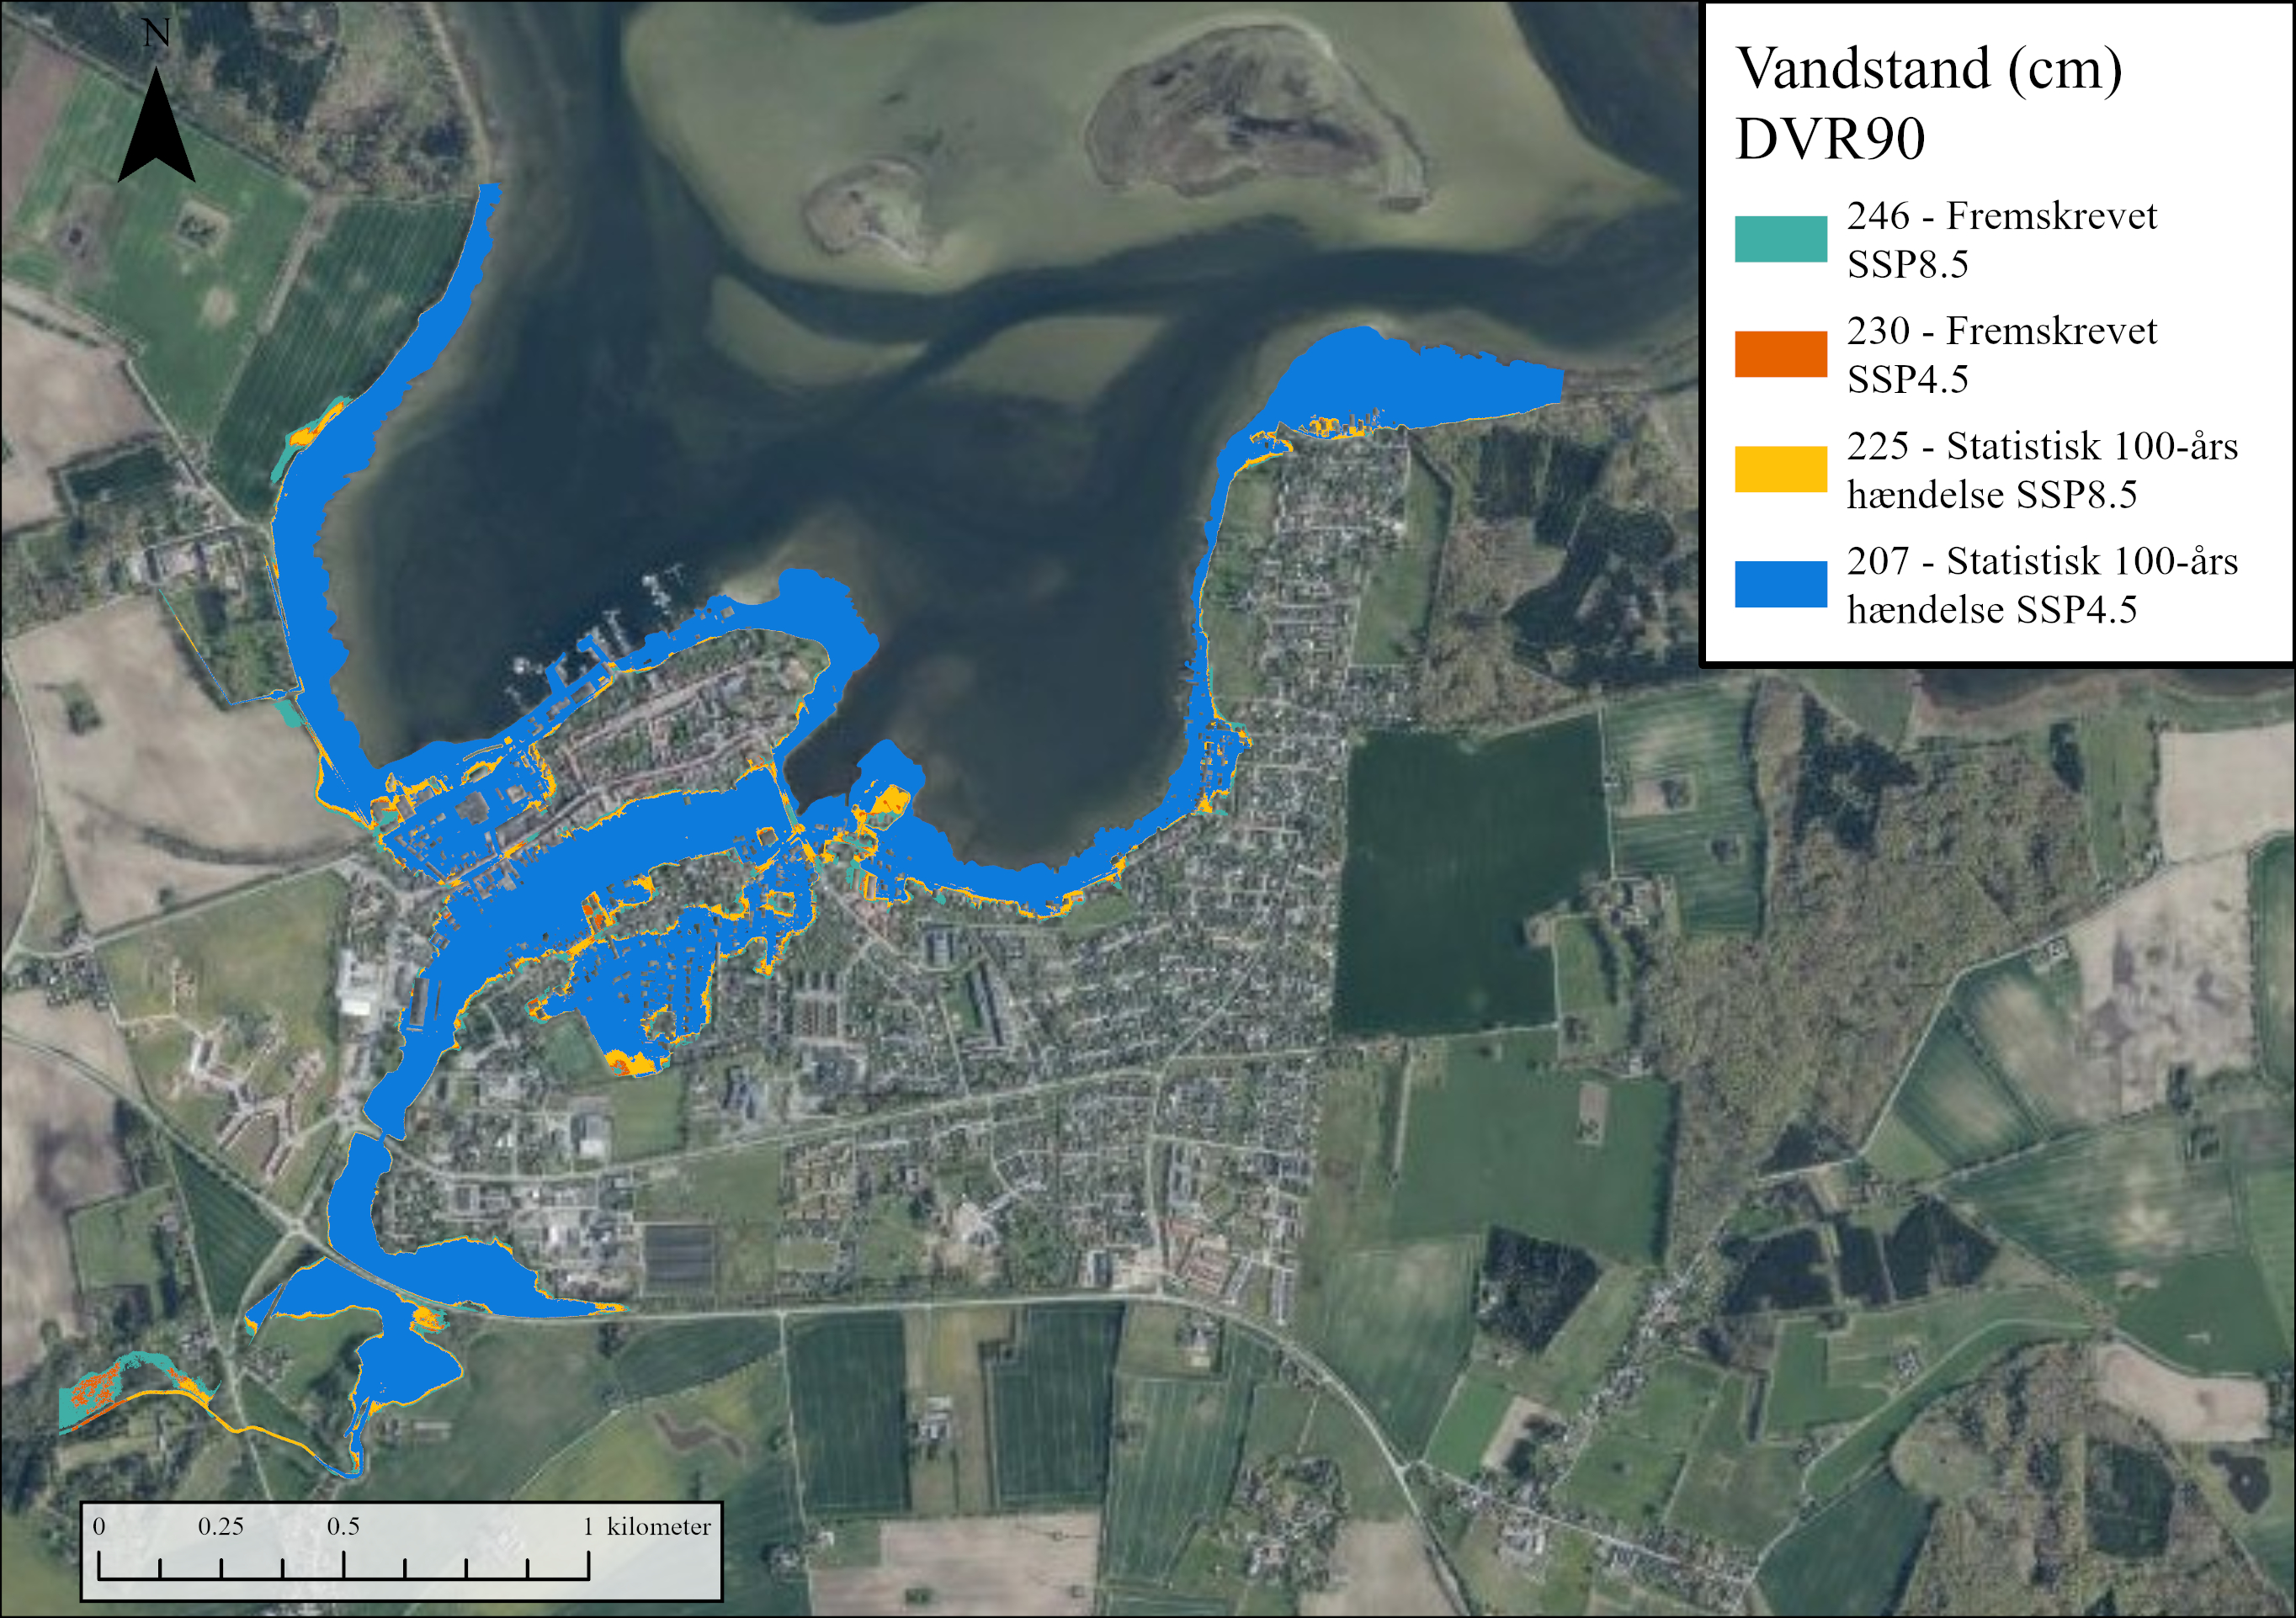
\includegraphics[width=0.8\linewidth]{images/Resultater/fremskrevet_hændelser/klima resultat praestoe.jpg}
    \caption{Kort over oversvømmet areal i Præstø af en stormflod ved en statistisk 100-års hændelse og en fremskrivning af oktober 2023 stormfloden til slutningen af århundredet ved SSP4,5 og SSP8,5 i centimeter over DVR90}
    \label{Figur: Klima Præstø}
\end{figure}

Sammenfattet bliver alle studieområderne i stor grad påvirket af oversvømmelser ved stormfloder. I tabel \ref{Tabel: Oversvømmet arealer af stormfloder} er der blevet kvantificeret størrelsen af oversvømmelserne i m\textsuperscript{2} for alle hændelser modelleret af Inundation Modellen samt den målte stormflod i 2023. Det største oversvømmet areal er i Gedser Havn ved en fremskrevet 2023 stormflod i SSP8,5 på 2180786,08 m\textsuperscript{2} og den mindste areal er simuleringen af 2023 stormfloden i Hesnæs på 32780,64 m\textsuperscript{2}. \\

\begin{table}[H]
\centering
\renewcommand{\arraystretch}{1.5} 
\begin{threeparttable}
\caption{Oversvømmet areal af den målte 2023 stormflod, den simuleret 2023 stormflod samt den statistiske 100-års hændelse og den fremskrevet 2023 stormflod til slutningen af århundredet ved SSP4.5 og 8.5 i m\textsuperscript{2} for hvert studieområde.}
\begin{tabular}{@{} l S[table-format=7.2, output-decimal-marker={,}] 
                    S[table-format=7.2, output-decimal-marker={,}] 
                    S[table-format=7.2, output-decimal-marker={,}] 
                    S[table-format=7.2, output-decimal-marker={,}] 
                    S[table-format=7.2, output-decimal-marker={,}] 
                    S[table-format=7.2, output-decimal-marker={,}] @{}} 
\toprule
& \multicolumn{1}{c}{\textbf{\makecell{Målt 2023\\stormflod}}} 
& \multicolumn{1}{c}{\textbf{\makecell{Simuleret 2023\\stormflod}}} 
& \multicolumn{2}{c}{\textbf{\makecell{Statistisk 100-års\\hændelse}}} 
& \multicolumn{2}{c}{\textbf{\makecell{Fremskrevet 2023\\stormflod}}} \\ 
\cmidrule(l){4-5} \cmidrule(l){6-7}
{\textit{m\textsuperscript{2}}} & & & {\textit{SSP4.5}} & {\textit{SSP8.5}} & {\textit{SSP4.5}} & {\textit{SSP8.5}} \\
\midrule
  Aabenraa & 707128,00 & 1297614,08 & 1552065,76 & 1666876,64 & 1666875,04 & 1748557,12 \\
  Gedser & 344734,72 & 331764,80 & 2051348,32 & 2196907,36 & 2010305,92 & 2180786,08 \\ 
  Hesnæs & 34572,16 & 32780,64 & 47723,36 & 1134312,48 & 48374,88 & 1147697,44 \\
  Præstø & 534967,2 & 398365,44 & 757009,92 & 820445,44 & 840784,32 & 897334,24 \\
\bottomrule
\end{tabular}
\label{Tabel: Oversvømmet arealer af stormfloder}
\end{threeparttable}
\end{table}

 